\documentclass[xcolor=svgnames]{beamer}
%\documentclass[dvipsnames]{beamer}
%\documentclass[dvipsnames,handout,draft]{beamer}

%\includeonly{introstorage}
%\includeonly{performancetuning}
%\includeonly{fileformats}
%\includeonly{datamanagement}
%\includeonly{conclusions}

\mode<presentation>{
  \usetheme{Madrid}
  \setbeamertemplate{navigation symbols}{} % suppress nav bar
%\logo{\pichere{\put(-55,-5){\includegraphics[scale=0.1]{scinet-logo.png}}}}
\logo{\pichere{\put(-50,-8){
\includegraphics[scale=0.45]{logos/hpcs2016}}}}
%\usecolortheme[named=RoyalBlue]{structure}
%\setbeamercolor*{alerted text}{fg=RoyalBlue}
\setbeamercolor*{alerted text}{fg=Blue}
}

\newcommand{\continue}{}


% set bold tt and math fonts
\font\ttbf = cmbtt10
\font\ttit = cmitt10
\font\ttrm = cmtt10
\let\tt=\ttbf
\boldmath

%command for "some identifier": an italic tt type
%\newcommand{\some}[1]{{\ttit #1}}
\newcommand{\some}[1]{{\ttrm #1}}
\newcommand{\dollar}{\mbox{\tt\small\$}}

%colors in code: ways to color
%\newcommand{\ftype}[1]   {\textcolor{OliveGreen}{\tt #1}} %for types
%\newcommand{\fns}[1]     {\textcolor{MidnightBlue}{#1}}   %for namespaces
%\newcommand{\fprec}[1]   {\textcolor{cyan}{#1}}           %for preprocessor   
%\newcommand{\fintr}[1]   {\textcolor{RedViolet}{#1}}      %for intrinsic keywords
%\newcommand{\fcomm}[1]   {\textcolor{MidnightBlue}{#1}}   %for comments
%\newcommand{\literal}[1] {\textcolor{brown}{#1}}          %for literals
%\newcommand{\fstring}[1] {\literal{"#1"}}                 %for strings
%keywords
\newcommand{\cunsigned}  {\ftype{unsigned}}
\newcommand{\cint}       {\ftype{int }}
\newcommand{\cvoid}      {\ftype{void }}
\newcommand{\clong}      {\ftype{long }}
\newcommand{\cshort}     {\ftype{short }}
\newcommand{\cfloat}     {\ftype{float }}
\newcommand{\cdouble}    {\ftype{double }}
\newcommand{\cchar}         {\ftype{char }}
\newcommand{\creturn}       {\fintr{\tt return }}
\newcommand{\cstruct}       {\fintr{\tt struct }}
\newcommand{\cenum}         {\fintr{\tt enum }}
\newcommand{\cunion}        {\fintr{\tt union }}
\newcommand{\cclass}        {\fintr{\tt class }}
\newcommand{\ctypedef}      {\fintr{\tt typedef }}
\newcommand{\cif}           {\fintr{\tt if }}
\newcommand{\celse}         {\fintr{\tt else }}
\newcommand{\cfor}          {\fintr{\tt for }}
\newcommand{\cnew}          {\fintr{\tt new }}
\newcommand{\cdelete}       {\fintr{\tt delete }}
\newcommand{\cswitch}       {\fintr{\tt switch }}
\newcommand{\ccase}         {\fintr{\tt case }}
\newcommand{\cdefault}      {\fintr{\tt default}}
\newcommand{\cbreak}        {\fintr{\tt break}}
\newcommand{\cwhile}        {\fintr{\tt while }}
\newcommand{\cdo}           {\fintr{\tt do }}
\newcommand{\cfriend}       {\fintr{\tt friend }}
\newcommand{\cvirtual}      {\fintr{\tt virtual }}
\newcommand{\cprivate}[1]   {\fintr{\tt private#1}}
\newcommand{\cpublic}[1]    {\fintr{\tt public#1}}
\newcommand{\cprotected}[1] {\fintr{\tt protected#1}}
\newcommand{\cpoundincludebrackets}[1]{\fprec{\tt\#include \literal{<#1>}}}
\newcommand{\cpoundinclude}[1]{\fprec{\tt\#include \literal{"#1"}}}


%%%%%%%%%%%%%%%%%%%%%%%%%%%%%%%%%%%%%%%%%%%%%%%%%%%%%%%%%%%%%%%%%%%%%


% colors in code: ways to color
\newcommand{\ftype}[1]   {\textcolor{OliveGreen}{\tt #1}} % for types
\newcommand{\fns}[1]     {\textcolor{MidnightBlue}{#1}}   % for namespaces
\newcommand{\fprec}[1]   {\textcolor{BlueViolet}{#1}}     % for preprocessor   
\newcommand{\fintr}[1]   {\textcolor{RedViolet}{#1}}      % for intrinsic keywords
\newcommand{\fcomm}[1]   {\textcolor{MidnightBlue}{#1}}   % for comments
\newcommand{\literal}[1] {\textcolor{brown}{#1}}          % for literals
\newcommand{\fstring}[1] {\literal{"#1"}}                 % for strings

\newcommand{\fred}[1] {\textcolor{red}{#1}}
\newcommand{\forangered}[1]{\textcolor{OrangeRed}{#1}}
\newcommand{\fredorange}[1]{\textcolor{RedOrange}{#1}}
\newcommand{\frawsienna}[1]{\textcolor{RawSienna}{#1}}
\newcommand{\femerald}[1]{\textcolor{Emerald}{#1}}
\newcommand{\fbrickred}[1]{\textcolor{BrickRed}{#1}}
\newcommand{\fpinegreen}[1]{\textcolor{PineGreen}{#1}}
\newcommand{\fplum}[1]{\textcolor{Plum}{#1}}

%\input{auxs/shellnewcommands}
%\input{auxs/cppnewcommands}
%\input{auxs/lstsettings}


%a tabbed code environment in  box:
%sample:
%\begin{code}
%   int main() 
%  \begin{bracing}
%      int z = 0;
%      for (int i=0;i<60;i++)
%      \begin{tab}
%             z+=i;
%      \end{tab}
%   \end{bracing}
%\end{code}
\usepackage{setspace}
\xdefinecolor{headerbgcolor} {rgb}  {0.84, 0.84, 0.94}
\newlength{\tbl}\tbl0pc
\newenvironment{tab}
{\par\addtolength\tbl{1.2pc}\leftskip\tbl\tt}
{\addtolength\tbl{-1.2pc}\par\leftskip\tbl\rm}
\newenvironment{bracing}{{\scriptsize$\{$}\begin{tab}}{\end{tab}{\scriptsize$\}$}}

\makeatletter
\newenvironment{code}
{\begin{lrbox}{\@tempboxa}\begin{minipage}{0.92\columnwidth}\setstretch{0.85} \tt \setlength{\rightskip}{-0.4pc}}
{\end{minipage}\end{lrbox}\par\centerline{\colorbox{headerbgcolor}{\colorbox{white}{\usebox{\@tempboxa}}}}\vspace{1mm}}
\makeatother

%puts a zero-sized picture command at the current point
\newcommand{\pichere}[1]{\begin{picture}(0,0)\thicklines #1\end{picture}}

%a block for gotcha's
\newenvironment{gotcha}[1][]{\begin{block}{\color{Yellow}Gotcha: #1}}{\end{block}}

%\colorbox{#1}{\textcolor{#2}

\newcommand{\mediumblue}{\color{Blue}}
\newcommand{\black}{\color{Black}}
\newcommand{\restpointslide}[1]{
  \frame{
    \begin{quote}
      \Large\bf\mediumblue #1
    \end{quote}
  }
}

\newenvironment{examplesegment}{\setbeamercolor{frametitle}{bg=ForestGreen}
\setbeamercolor{block title}{bg=ForestGreen}
\setbeamercolor*{alerted text}{fg=Black}
\setbeamerfont{alerted text}{series=\bfseries}
\renewcommand{\mediumblue}{\color{ForestGreen}}}
{\setbeamercolor{frametitle}{bg=Blue}
\setbeamercolor{block title}{bg=Blue}
\setbeamercolor*{alerted text}{fg=Blue}
\setbeamerfont{alerted text}{series=\rmseries}
\renewcommand{\mediumblue}{\color{Blue}}}

\newenvironment{handsonsegment}{\setbeamercolor{frametitle}{bg=OrangeRed}
\setbeamercolor{block title}{bg=OrangeRed}
\setbeamercolor*{alerted text}{fg=Black}
\setbeamerfont{alerted text}{series=\bfseries}
\renewcommand{\mediumblue}{\color{OrangeRed}}}
{\setbeamercolor{frametitle}{bg=Blue}
\setbeamercolor{block title}{bg=Blue}
\setbeamercolor*{alerted text}{fg=Blue}
\setbeamerfont{alerted text}{series=\rmseries}
\renewcommand{\mediumblue}{\color{Blue}}}


% INTROD
%%%%
\newcommand{\introEnv}{
  \colorlet{mystruct}{structure}
  %\colorlet{structure}{magenta}
  \usestructuretemplate{\color{structure}}{} \beamertemplateshadingbackground{gray!30}{lightgray!30}
}
%%%%


% normal
%%%%
\newcommand{\normEnv}{
  \colorlet{mystruct}{structure}
  %\colorlet{structure}{magenta}
  \usestructuretemplate{\color{structure}}{} \beamertemplateshadingbackground{orange!10}{blue!10}
}
%%%%

% RESET
%%%%
\newcommand{\resetEnv}{
  \colorlet{structure}{mystruct}
  \beamertemplateshadingbackground{blue!5}{gray!10}
  \beamertemplateshadingbackground{white}{white}
}
%%%%

% ADVANCED
%%%%
\newcommand{\advEnv}{
  \colorlet{mystruct}{structure}
  %\colorlet{structure}{magenta}
  \usestructuretemplate{\color{structure}}{} \beamertemplateshadingbackground{orange!25}{blue!30}
}
%%%%


% normal2
%%%%
\newcommand{\normalEnv}{
  \colorlet{mystruct}{structure}
  %\colorlet{structure}{magenta}
  \usestructuretemplate{\color{structure}}{} \beamertemplateshadingbackground{red!20}{blue!20}
}
%%%%


% BASIC
%%%%
\newcommand{\basicEnv}{
  \colorlet{mystruct}{structure}
  %\colorlet{structure}{magenta}
  \usestructuretemplate{\color{structure}}{} \beamertemplateshadingbackground{red!10}{blue!10}
}
%%%%


%\usepackage{chemarrow}
\usepackage{mathtools}
\usepackage{pifont} % required for use "\ding{}" in 'miktex'

\usepackage{xcolor}


\usepackage{verbatim}
\usepackage{listings}



%\providecommand{\sectionpage}{\Large\centering Section \thesection\par\ \vspace{-2mm}\\ \bf\mediumblue\insertsection}
\providecommand{\sectionpage}{\Large\centering \bf\mediumblue\insertsection}
\def\ra{$\rightarrow$\,\,}
\definecolor{cadet}{rgb}{0.33, 0.41, 0.47}
\newcommand{\hi}[1]{{\color{cadet}\textsl{#1}}}


\begin{document}
%%%%%%%%%%%%%%%%%%%%%%%%%%%%%%%%%%%%%%%%%%%%%%%%%%%%%%%%%%%%%%%%%%%%%
\title[VisIt Workshop]{\Large\bf Scientific Visualization using VisIt}
\author[\textbf{M.Ponce} \& \textbf{A.Razoumov}]{\Large {\sc Marcelo Ponce}~~~and~~~{\sc Alex Razoumov}}
\date[HPCS 2016]{HPCS 2016 -- Edmonton, AB \\ June 20th, 2016 \\ /*~~\textcolor{DarkRed}{\small slides and data files at \textcolor{DarkBlue}{\url{http://bit.ly/visitfiles}}}~~*/}
\institute[SciNet/WestGrid]{
\includegraphics[width=0.35\columnwidth]{./logos/SciNet_newLogo}\hspace{.65cm}
\includegraphics[width=0.45\columnwidth]{./logos/WG-Logo-Jan16}}
%%%%%%%%%%%%%%%%%%%%%%%%%%%%%%%%%%%%%%%%%%%%%%%%%%%%%%%%%%%%%%%%%%%%%

\begin{frame}
  \centering
%  \includegraphics[width=11cm,height=5cm]{logos/ohpcss}
\href{https://wci.llnl.gov/simulation/computer-codes/visit/}{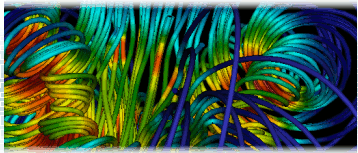
\includegraphics[height=1.15cm]{./figs/visit-logos/VisIt-01}} \href{https://wci.llnl.gov/simulation/computer-codes/visit/}{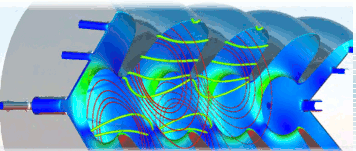
\includegraphics[height=1.15cm]{./figs/visit-logos/VisIt-02}} \href{https://wci.llnl.gov/simulation/computer-codes/visit/}{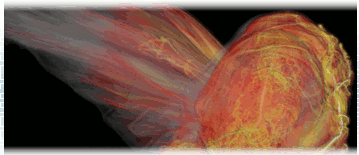
\includegraphics[height=1.15cm]{./figs/visit-logos/VisIt-03}} \href{https://wci.llnl.gov/simulation/computer-codes/visit/}{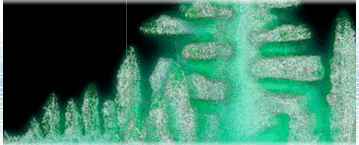
\includegraphics[height=1.15cm]{./figs/visit-logos/VisIt-04}}

  \vspace{-.25cm}

  \titlepage
\end{frame}

%%%%%%%%%%%%%%%%%%%%%%%%%%%%%%%%%%%%%%%%%%%%%%%%%%%%%%%%%%%%%%%%%%%%%
\begin{frame}[shrink=0.9]
\frametitle{Outline of the workshop}

\vspace{-5mm}
%\begin{columns}[T]
%\begin{column}{5.5cm}
%  \begin{block}{Topics to cover:}
%    \begin{itemize}\itemsep3pt
%	\item A quick introduction to Visualization \& VisIt
%	\item GUIs overview
%	\item accessing data and managing files
%	\item client/server visualization
%	\item working with plots%: overview, pseudocolour, mesh, filled boundary, boundary, contour, volume, vector, subset, streamline, curve, histogram, lable, molecule, truecolour, scatter, spreadsheet, parallel coordinates
	%\item using the visualization window
%	\item viz pipeline: working with operators%: overview, slice, reflect, clip, transform, data binning, threshold, isosurface, isovolume, elevate, replicate, resample, displace, index select, box, three slice, cylinder, inverse ghost zone, spherical slice
%	\item interactive tools%: box, line, plane, sphere, point, axis restriction
	%\item subsets
%	\item quantitative analysis
	%\item making it pretty
%	\item animation and keyframing
%	\item scripting 
%    \end{itemize}
%  \end{block}
%\end{column}
%\begin{column}{5.5cm}
 %  \begin{block}{Table of Contents}%\itemsep8pt
%  \begin{beamerboxesrounded}{Table of Contents}
  %\vspace{2.5mm}
  %\setcounter{tocdepth}{1}
  %\setcounter{secnumdepth}{1}
  %\begin{spacing}{-.5}
	\tableofcontents[hideallsubsections]%[currentsection,currentsubsection]
  %\end{spacing}
%  \end{beamerboxesrounded}
 %  \end{block}
%\end{column}
%\end{columns}
\end{frame}

%%%%%%%%%%%%%%%%%%%%%%%%%%%%%%%%%%%%%%%%%%%%%%%%%%%%%%%%%%%%%%%%%%%
%mp Marcelo
\section{Introduction to Visualization}
\introEnv
\frame{\sectionpage}
%%%%
  

\section{Scientific Visualization}
\subsection{Generalities}
\begin{frame}
    \frametitle{Scientific Visualization}
    \framesubtitle{}

    \vspace{-2.5mm}
    \begin{columns} %[T]
    \begin{column}{5.325cm}
        \begin{itemize}
                \item represent data
                \item plotting
                \item visualization techniques
                \item analyze/explore
                \item communicate (publications/talks)
                \item make it look nice?
        \end{itemize}

        \centering
        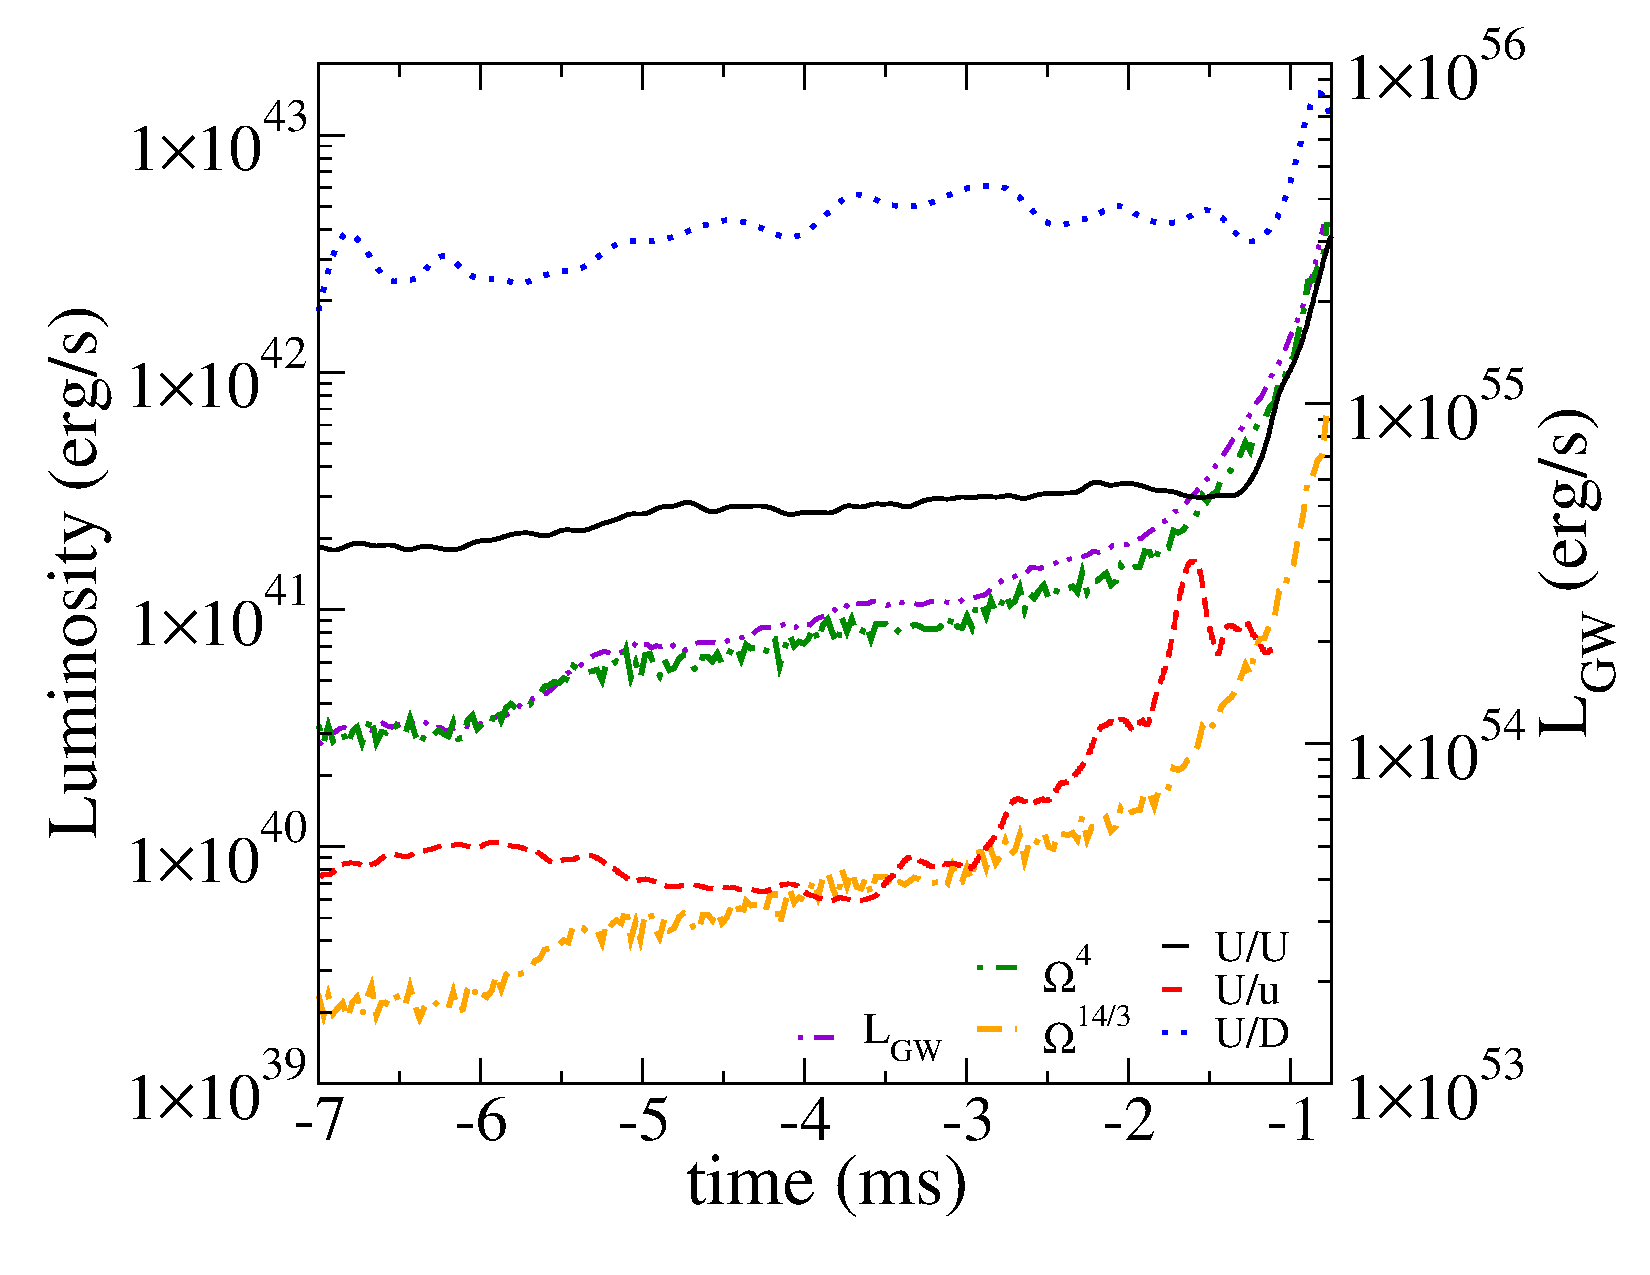
\includegraphics[width=.5\columnwidth]{plots/mpc/figure3_B}

        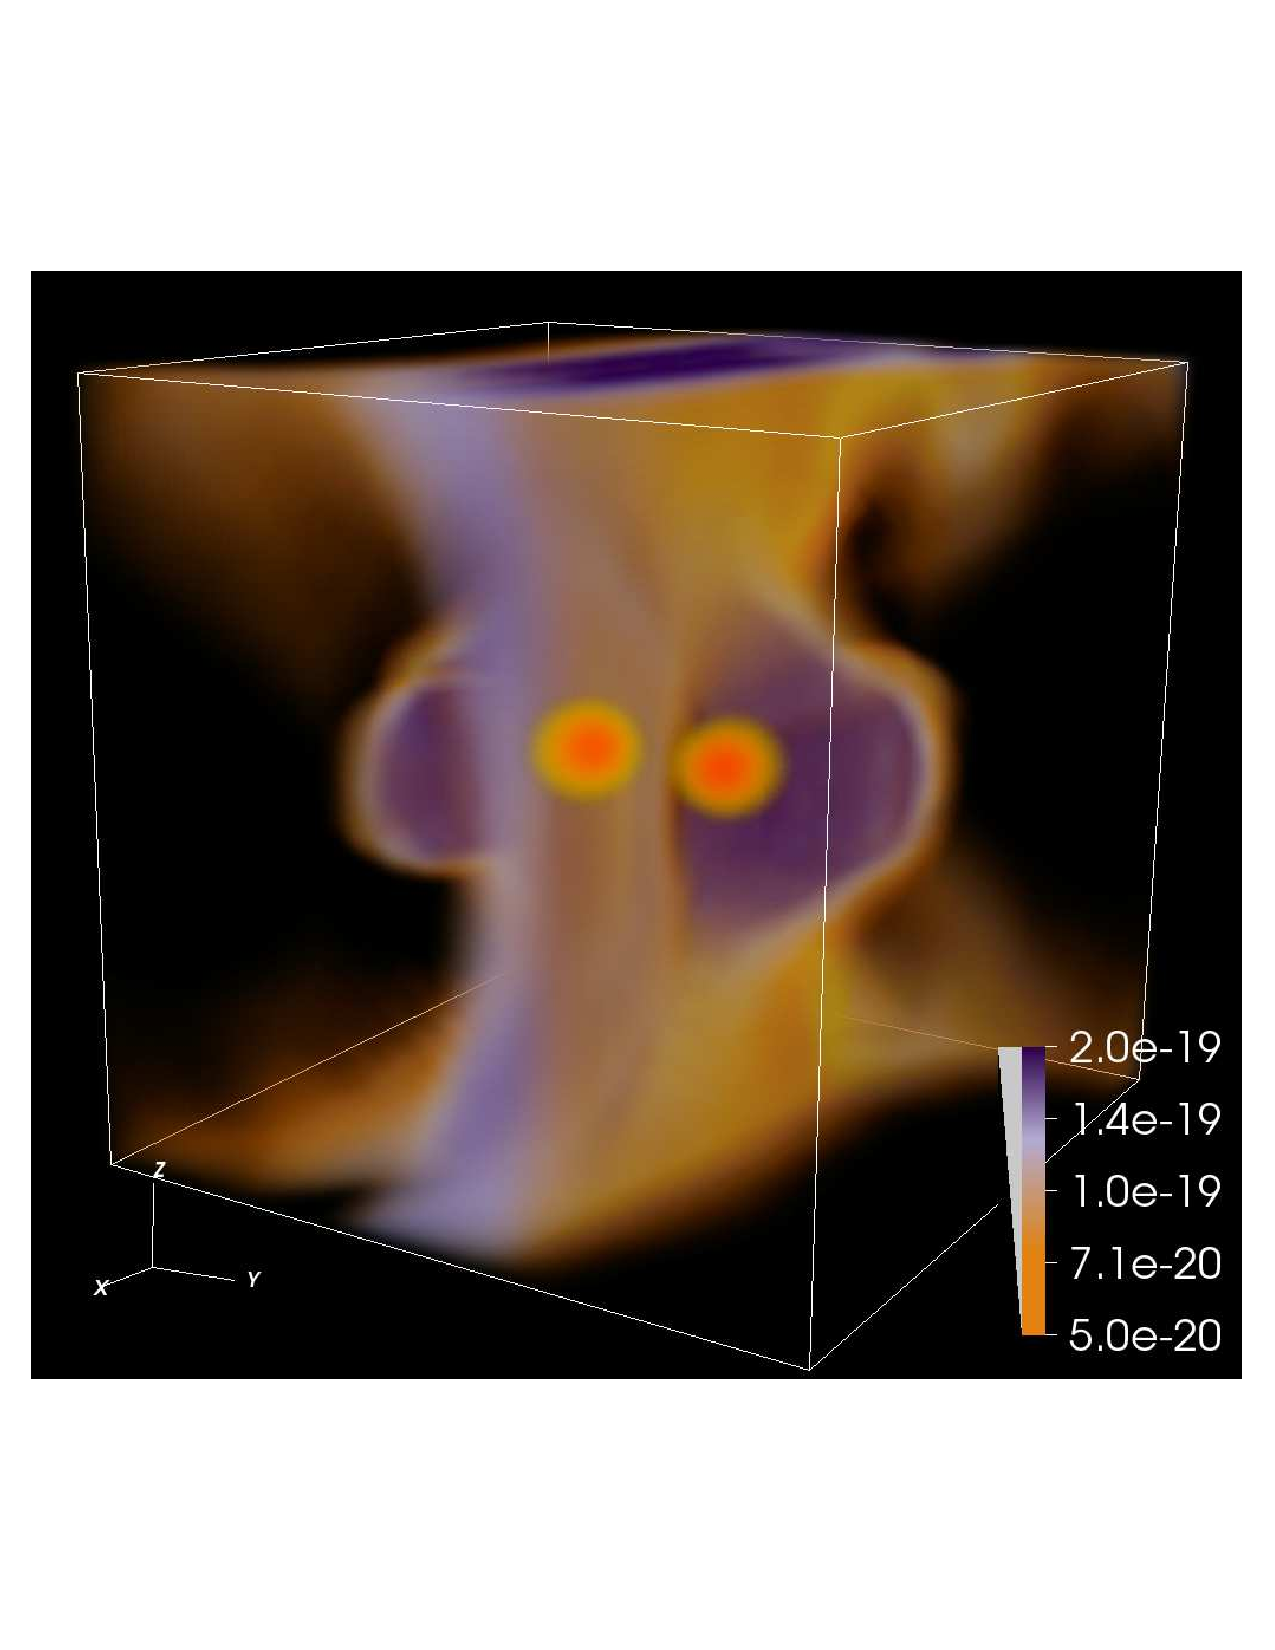
\includegraphics[width=0.33\columnwidth]{plots/mpc/bns01_UU-sqphi2_3d-14b}
        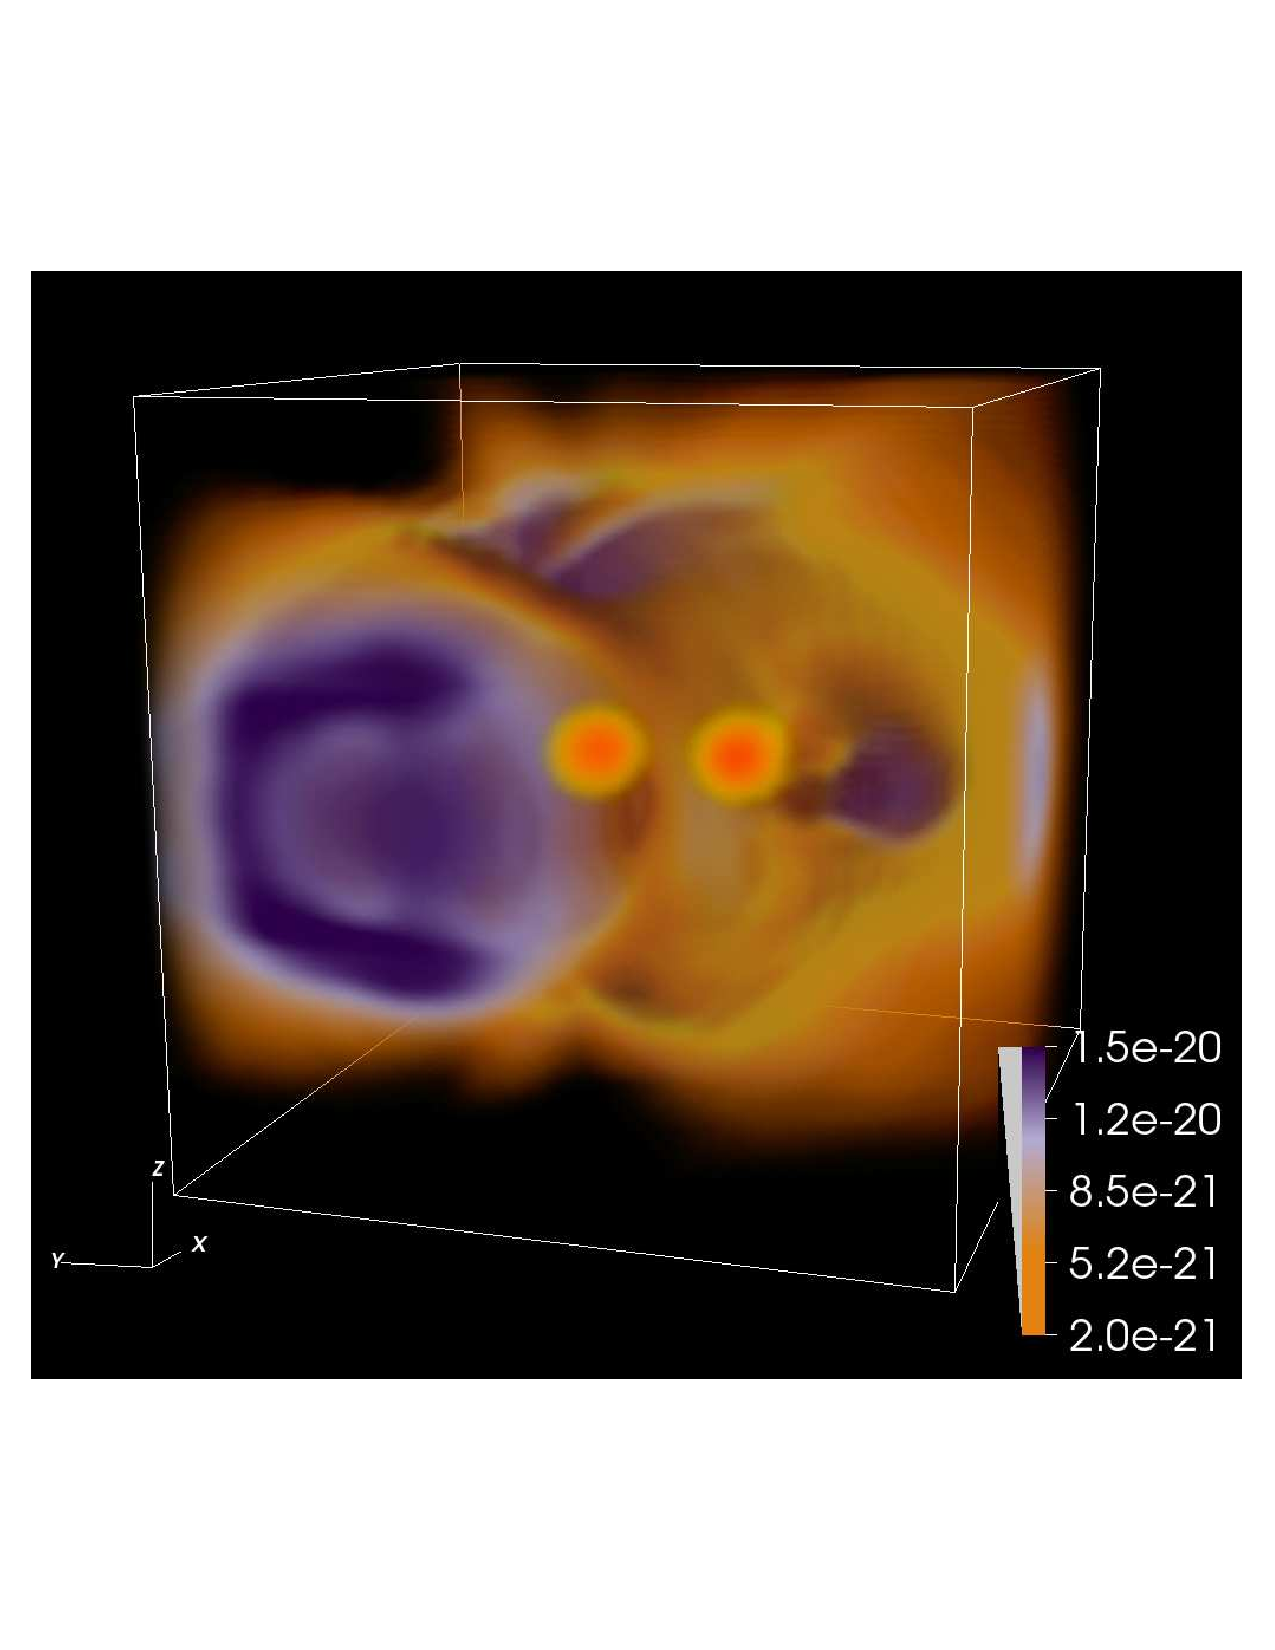
\includegraphics[width=0.33\columnwidth]{plots/mpc/bns02_Uu-sqphi2_3d-14c}
        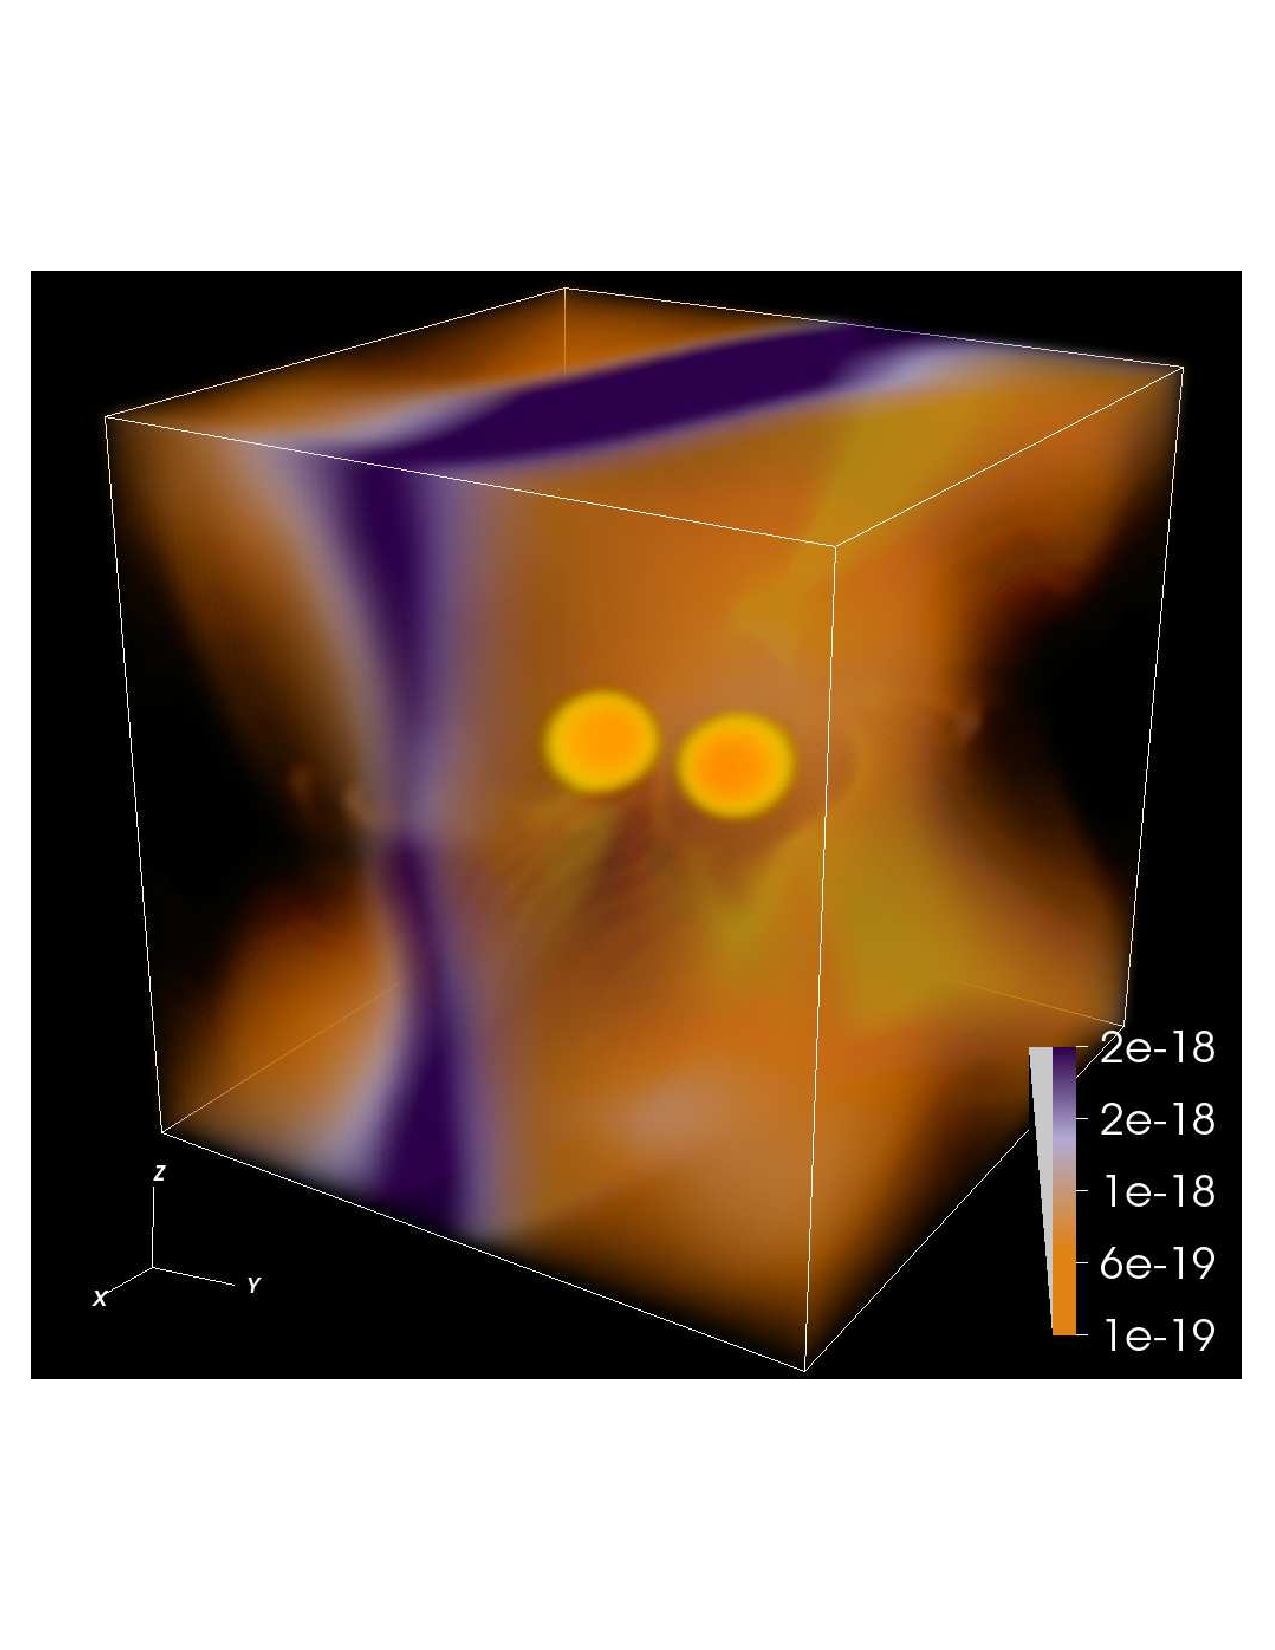
\includegraphics[width=0.33\columnwidth]{plots/mpc/bns03_UD-sqphi2_3d-14b}
    \end{column}
    \begin{column}{7.5cm}
        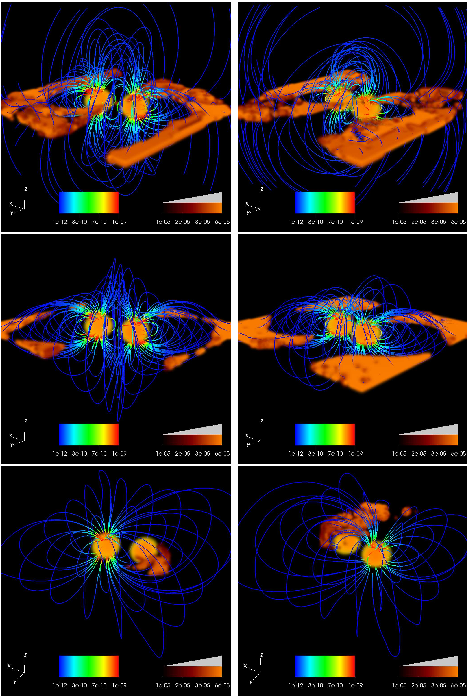
\includegraphics[width=\columnwidth,clip=true,trim=0 4cm 0 4cm]{plots/mpc/plot_Bxi}
        %
        %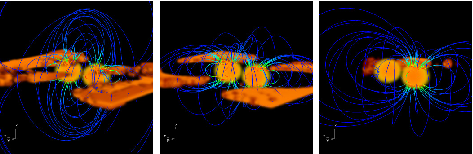
\includegraphics[width=\columnwidth]{plots/mpc/figure1_c}
        \\
        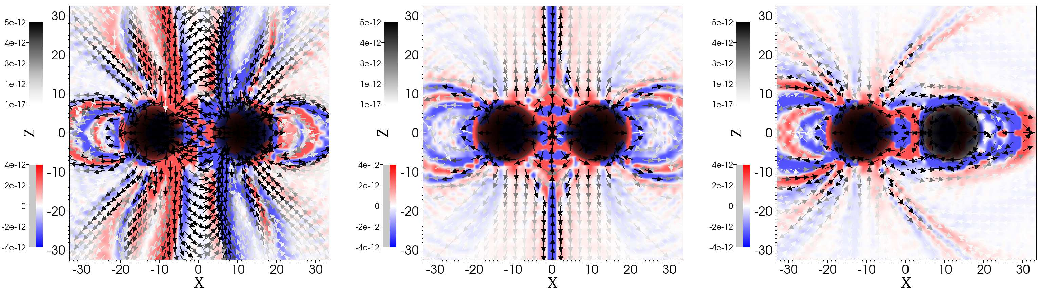
\includegraphics[width=\columnwidth]{plots/mpc/plot_current}
        \\
        %\href{http://journals.aps.org/prd/kaleidoscope/}{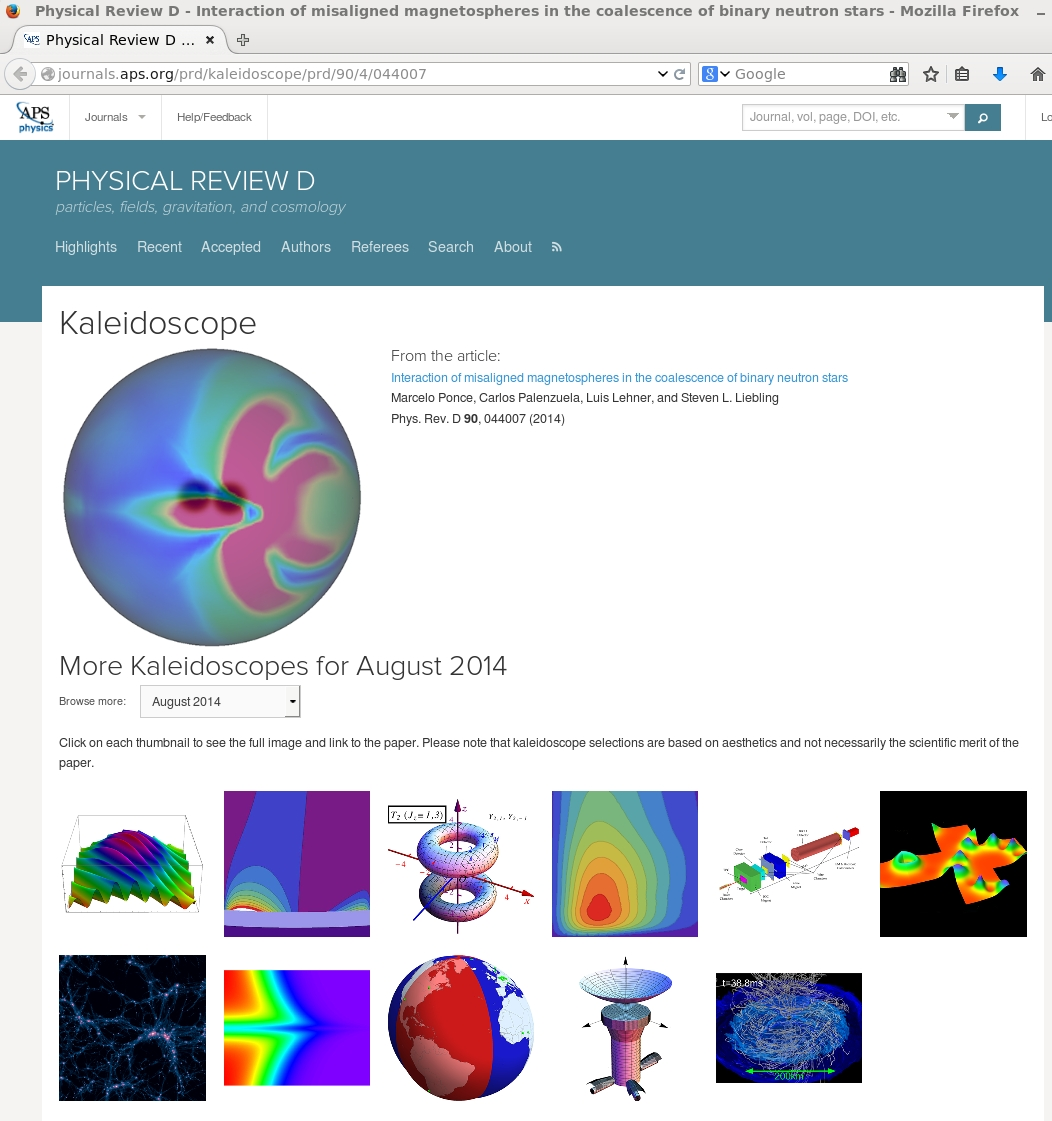
\includegraphics[width=\columnwidth, clip=true,trim=1.25cm 3.5mm 3.5mm 19.75cm]{plots/mpc/kaleidoscope}
        \href{http://journals.aps.org/prd/kaleidoscope/August2014}{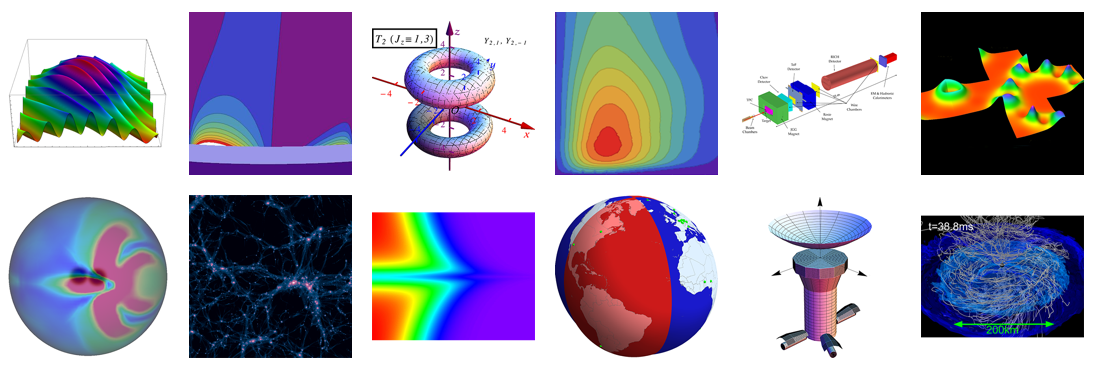
\includegraphics[width=\columnwidth]{plots/mpc/kaleidoscope_aug2014}}
    \end{column}
    \end{columns}
\end{frame}


\subsection{2D/3D Visualization Generalities}
\begin{frame}
    \frametitle{}
    \framesubtitle{}

    \begin{columns} %[T]
    \begin{column}{5.25cm}
        \begin{itemize}
                \item \textcolor{DarkBlue}{Visualization} is the process of mapping scientific data into ``{\it visual form}''
                \item Much easier to understand images than a large set of numbers
                \item For interactive data exploration, debugging, communication with peers
        \end{itemize}
    \end{column}
    \begin{column}{7cm}
        \href{http://www.paraview.org/gallery/}{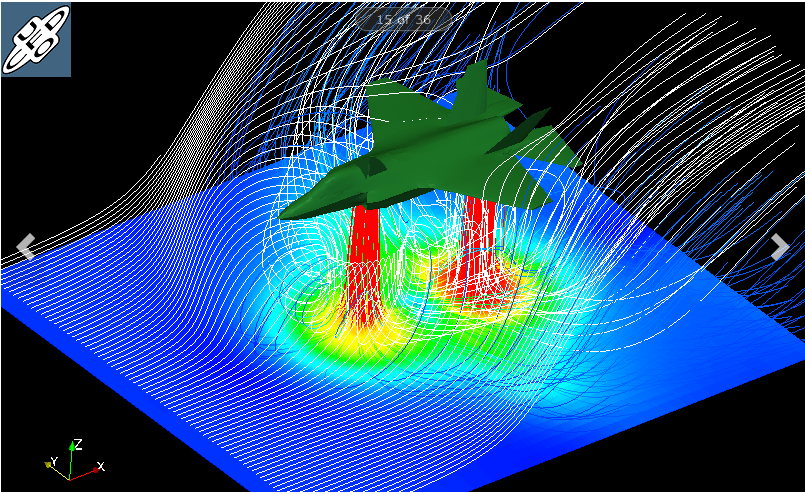
\includegraphics[width=.475\columnwidth]{figs/ParaView-gallery01}}
        \href{http://www.paraview.org/gallery/}{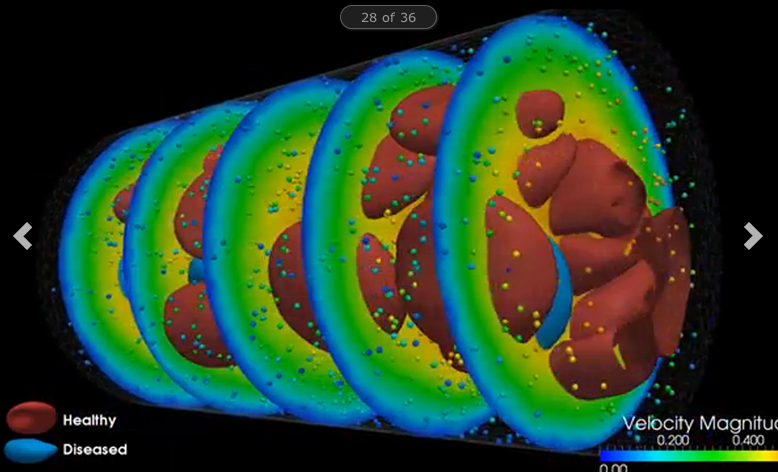
\includegraphics[width=.475\columnwidth]{figs/ParaView-gallery03}}
        \centering
        \href{http://www.paraview.org}{
\includegraphics[width=.45\columnwidth]{./figs/visit-logos//ParaViewLogo}}


        \href{https://wci.llnl.gov/simulation/computer-codes/visit/gallery}{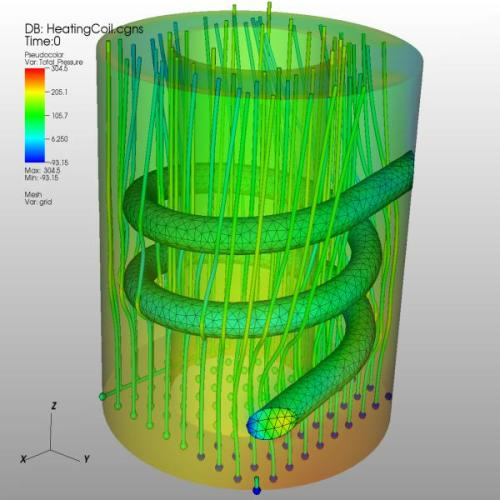
\includegraphics[width=.475\columnwidth]{figs/VisIt-gallery_12}}
        \href{https://wci.llnl.gov/simulation/computer-codes/visit/gallery}{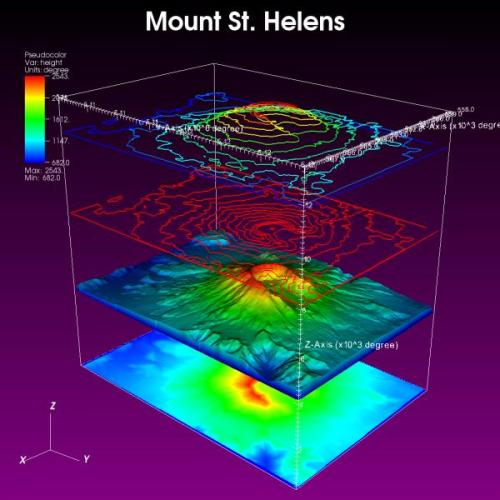
\includegraphics[width=.475\columnwidth]{figs/VisIt-gallery_15}}

        \centering
        \href{https://wci.llnl.gov/simulation/computer-codes/visit/}{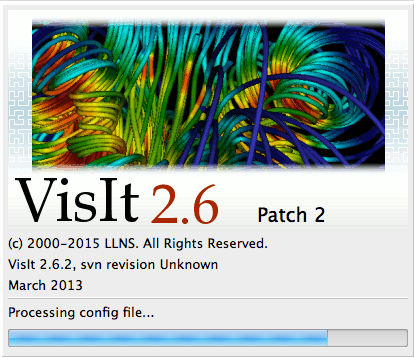
\includegraphics[width=.45\columnwidth, clip=true,trim=0 2cm 0 0]{./figs/visit-logos//VisIt26}}
    \end{column}
    \end{columns}


%    \begin{columns} %[T]
%    \begin{column}{5.5cm}
%       \centering
%       \href{https://wci.llnl.gov/simulation/computer-codes/visit/}{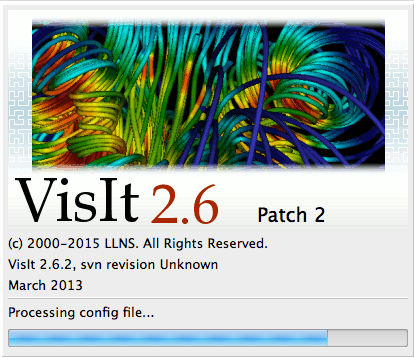
\includegraphics[width=.75\columnwidth, clip=true,trim=0 2cm 0 0]{./figs/visit-logos//VisIt26}}
%    \end{column}
%    \begin{column}{5.5cm}
%       \centering
%       \href{http://www.paraview.org}{
\includegraphics[width=.7\columnwidth]{./figs/visit-logos//ParaViewLogo}}
%    \end{column}
%    \end{columns}

\end{frame}


\begin{frame}
\frametitle{1D plotting vs. 2D/3D visualization}

\begin{columns}
\begin{column}{7cm}
\begin{beamerboxesrounded}[upper=block head,lower=block body,shadow=true]{\textcolor{DarkBlue}{\ding{232}} \textcolor{DarkGreen}{1D plotting}}
         plotting functions of one variable, 1D tabulated data (eg. \textcolor{DarkBlue}{\tt gnuplot},  \textcolor{DarkBlue}{\tt xmgr}, or Python's \textcolor{DarkRed}{\tt matplotlib} library)
\end{beamerboxesrounded}
\end{column}
\begin{column}{5cm}
        \centering
        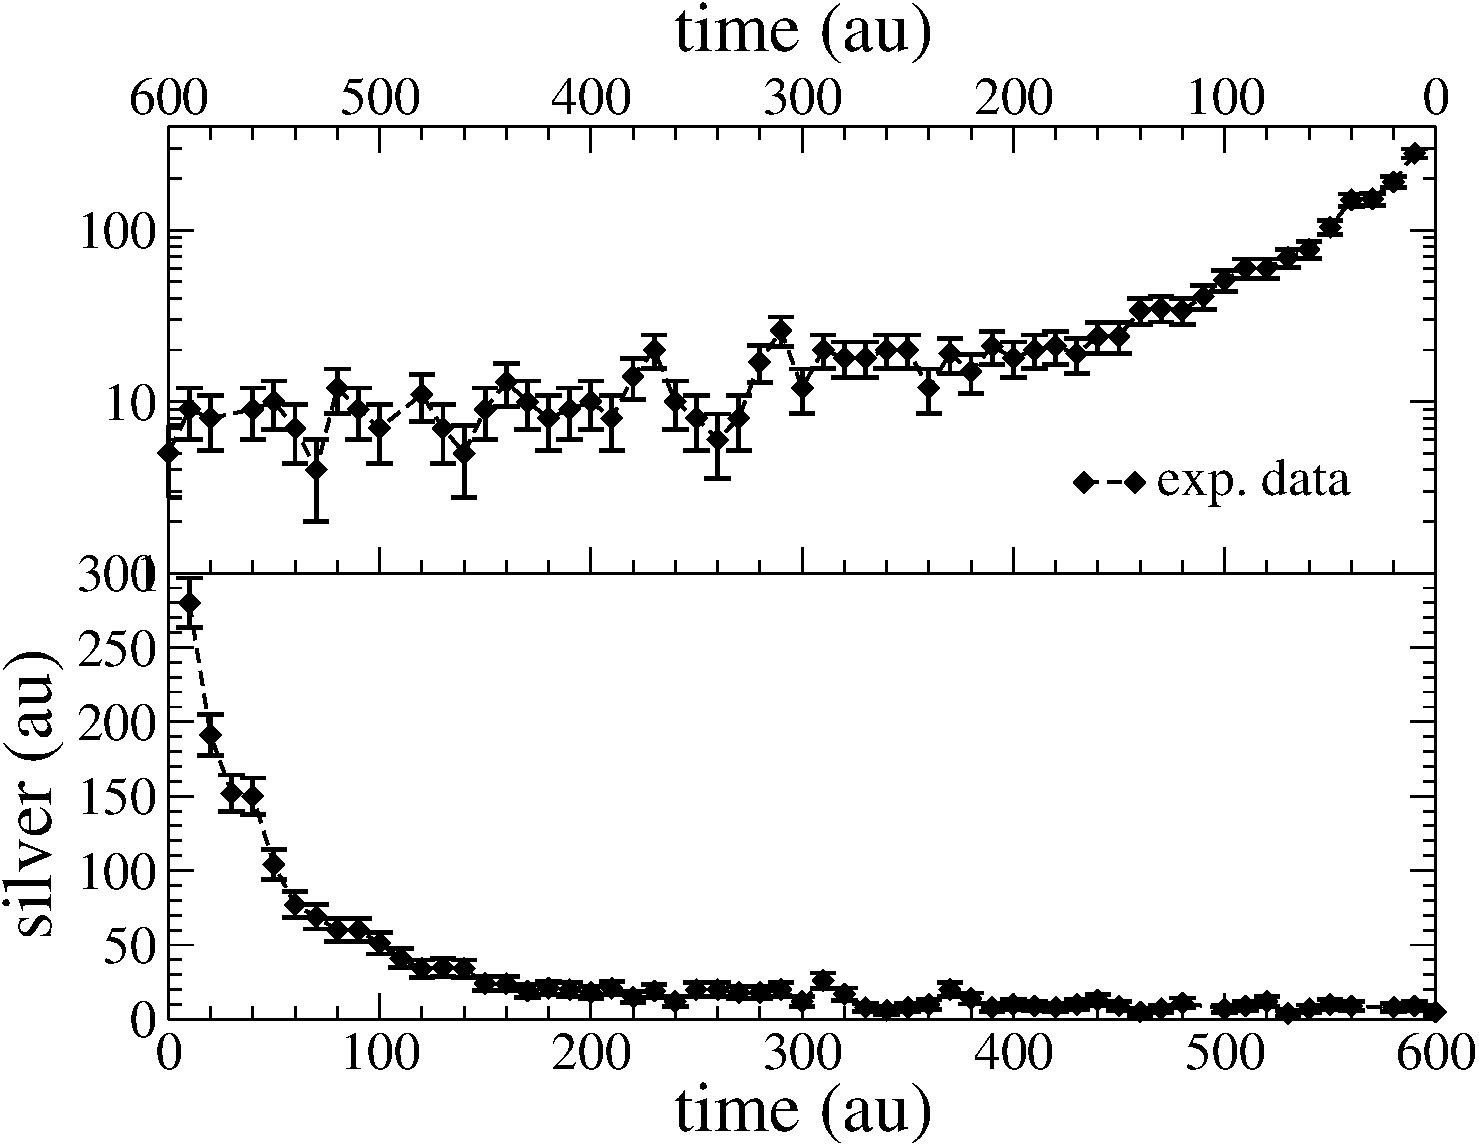
\includegraphics[width=.85\columnwidth]{plots/xmgr/silver_2plots}
\end{column}
\end{columns}

\begin{columns}
\begin{column}{7cm}
\begin{beamerboxesrounded}[upper=block head,lower=block body,shadow=true]{\textcolor{DarkBlue}{\ding{232}} \textcolor{DarkOrange}{2D/3D visualization} }
        displaying multi-dimensional datasets, typically
data on 2D/3D structured grids or on unstructured meshes (that have
some topology in 2D/3D)
\end{beamerboxesrounded}
\end{column}
\begin{column}{5cm}
        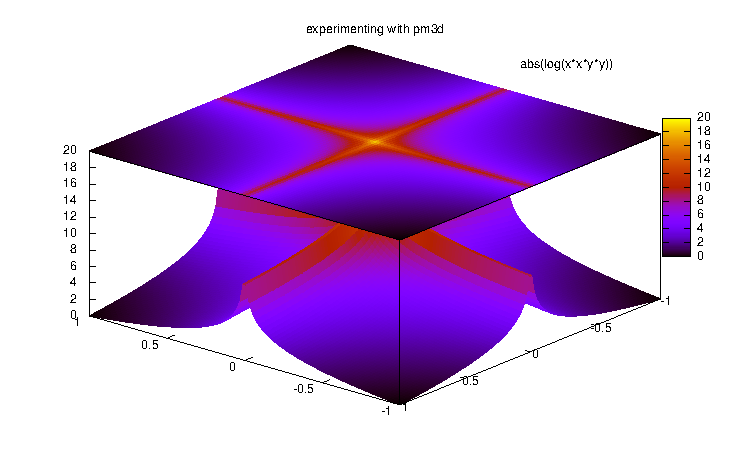
\includegraphics[width=1.1\columnwidth]{figs/others/pm3dplot}
\end{column}
\end{columns}

%Whatever you do, may be a good idea to avoid proprietary tools, unless those tools provide a clear advantage (most likely not)
%\begin{itemize}
%       \item large \$\$
%       \item limitations on where you can run them, which machines/platforms, etc.
%       \item cannot get help from open-source community, user base usually smaller than for open-source tools
%       \item once you start accumulating scripts, you lock yourself into using these tools forever, and consequently paying \$\$ on a regular basis
%       \item there is nothing you cannot do with open-source tools
%\end{itemize}
\end{frame}


\begin{frame}
\frametitle{2D/3D visualization packages}

\begin{small}
\vspace{-2mm}
%\begin{beamerboxesrounded}[upper=block head,lower=block body,shadow=true]{
\textcolor{DarkRed}{\ding{232}} \textcolor{DarkBlue}{\tt gnuplot}: %}
        command-driven interactive 2d and 3d plotting program
%\end{beamerboxesrounded}

\vspace{1.15mm}
%\begin{beamerboxesrounded}[upper=block head,lower=block body,shadow=true]{
\textcolor{DarkRed}{\ding{232}} \textcolor{DarkBlue}{\tt GraphViz}: %}
        represent strucrural information as diagrams of abstract graphs and networks
%\end{beamerboxesrounded}

\vspace{1.15mm}
%\begin{beamerboxesrounded}[upper=block head,lower=block body,shadow=true]{
\textcolor{DarkRed}{\ding{232}} \textcolor{DarkBlue}{\tt HDFview}: %}
        visual tool for browsing and editing HDF4 and HDF5 files
%\end{beamerboxesrounded}

\vspace{1.15mm}
%\begin{beamerboxesrounded}[upper=block head,lower=block body,shadow=true]{
\textcolor{DarkRed}{\ding{232}} \textcolor{DarkBlue}{\tt ImageMagick}: %}
        manipulation of image
%\end{beamerboxesrounded}

\vspace{1.15mm}
%\begin{beamerboxesrounded}[upper=block head,lower=block body,shadow=true]{
\textcolor{DarkRed}{\ding{232}} \textcolor{DarkBlue}{\tt Molden}: %}
        pre/post-processing for molecular and electronic structures
%\end{beamerboxesrounded}

\vspace{1.15mm}
%\begin{beamerboxesrounded}[upper=block head,lower=block body,shadow=true]{
\textcolor{DarkRed}{\ding{232}} \textcolor{DarkBlue}{\tt OpenCV}: %}
        library for real time computer vision
%\end{beamerboxesrounded}

%\vspace{1.15mm}
\begin{beamerboxesrounded}[upper=block head,lower=block body,shadow=true]{}
\textcolor{DarkRed}{\ding{232}} \textcolor{DarkBlue}{\tt ParaView}: %}
        Parallel visualization application
\end{beamerboxesrounded}

%\vspace{1.15mm}
%\begin{beamerboxesrounded}[upper=block head,lower=block body,shadow=true]{
\textcolor{DarkRed}{\ding{232}} \textcolor{DarkBlue}{\tt SciLab}: %}
        open source platform for numerical computation
%\end{beamerboxesrounded}

%\vspace{1.15mm}
\begin{beamerboxesrounded}[upper=block head,lower=block body,shadow=true]{}
\textcolor{DarkRed}{\ding{232}} \textcolor{DarkBlue}{\tt VisIt}: %}
        Visualization Tool for HPC
\end{beamerboxesrounded}

%\vspace{1.15mm}
%\begin{beamerboxesrounded}[upper=block head,lower=block body,shadow=true]{
\textcolor{DarkRed}{\ding{232}} \textcolor{DarkBlue}{\tt XCrysDen}: %}
        Crystaline and Molecular Structure Visualization
%\end{beamerboxesrounded}

\vspace{1.15mm}
%\begin{beamerboxesrounded}[upper=block head,lower=block body,shadow=true]{
\textcolor{DarkRed}{\ding{232}} \textcolor{DarkBlue}{\tt yt}: %}
        python-based package for visualization of AMR datasets
%\end{beamerboxesrounded}

\vspace{1.15mm}
%\begin{beamerboxesrounded}[upper=block head,lower=block body,shadow=true]{
\textcolor{DarkRed}{\ding{232}} \textcolor{DarkBlue}{\tt VMD}: %}
        Visualization for Molecular Dynamics
%\end{beamerboxesrounded}

%\vspace{1.15mm}
%\begin{beamerboxesrounded}[upper=block head,lower=block body,shadow=true]{
\textcolor{DarkRed}{\ding{232}} \textcolor{DarkBlue}{\tt openDX}: %}
        very old, not mantained package, but really \\nice approach to visualization process (modules)
%\end{beamerboxesrounded}
\end{small}
\end{frame}


\begin{frame}
\frametitle{2D/3D visualization packages}
\framesubtitle{General Features}

\begin{itemize}
        \item visualize \textcolor{DarkBlue}{scalar} and \textcolor{DarkBlue}{vector fields}
        \item \textcolor{DarkBlue}{structured and unstructured meshes} in 2D and 3D, particle data, polygonal
data, \textcolor{DarkBlue}{irregular topologies}
        \item ability to handle very \textcolor{DarkBlue}{large datasets} (GBs to TBs)
        \item ability to scale to large ($10^3 - 10^5$ cores) computing facilities
        \item \textcolor{DarkBlue}{iteractive manipulation}
        \item support for \textcolor{DarkBlue}{scripting}, \textcolor{DarkBlue}{common data formats}, \textcolor{DarkBlue}{parallel I/O}
        \item open-source, \textcolor{DarkBlue}{multi-platform}, and \textcolor{DarkBlue}{general-purpose}
\end{itemize}

    \begin{columns} %[T]
    \begin{column}{5.5cm}
        \centering
        \href{https://wci.llnl.gov/simulation/computer-codes/visit/}{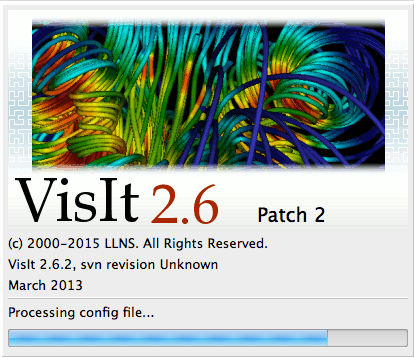
\includegraphics[width=.75\columnwidth, clip=true,trim=0 2cm 0 0]{./figs/visit-logos//VisIt26}}
    \end{column}
    \begin{column}{5.5cm}
        \centering
        \href{http://www.paraview.org}{
\includegraphics[width=.7\columnwidth]{./figs/visit-logos//ParaViewLogo}}
    \end{column}
    \end{columns}

\end{frame}



\subsection{Visualization Pipeline}
\begin{frame}

\begin{columns}
\begin{column}{8cm}
        \begin{beamerboxesrounded}[upper=block head,lower=block body,shadow=true]{\textcolor{DarkBlue}{\ding{231}} Data Visualization Process}
                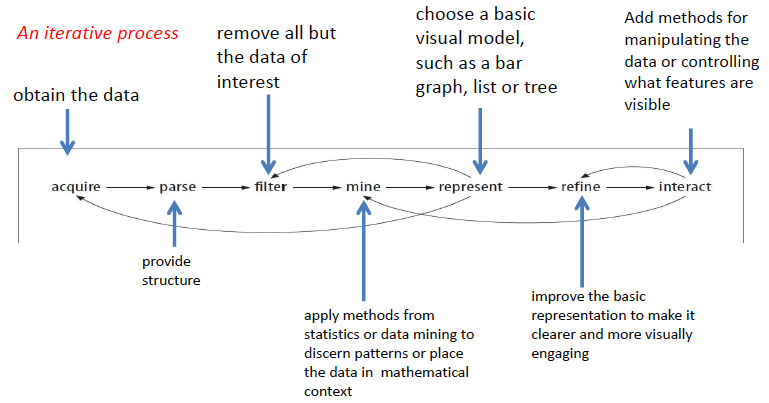
\includegraphics[width=\columnwidth]{figs/viz/viz_pipeline-loop}
        \end{beamerboxesrounded}
\end{column}
\begin{column}{4.5cm}
        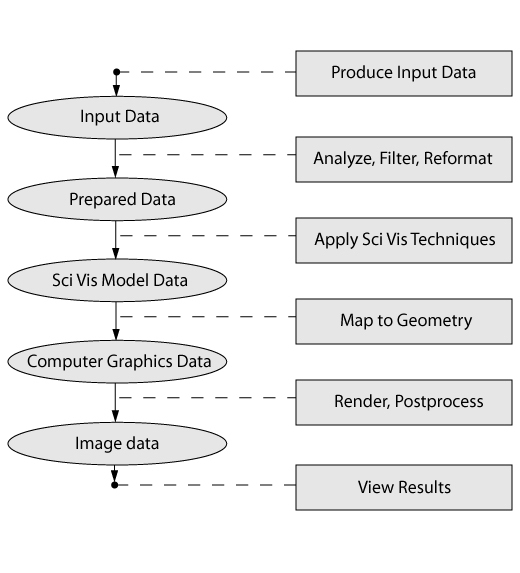
\includegraphics[width=\columnwidth]{figs/viz/viz-pipeline4}
\end{column}
\end{columns}

\begin{small}
\begin{columns}
\begin{column}{3.85cm}
\begin{beamerboxesrounded}[upper=block head,lower=block body,shadow=true]{\textcolor{DarkRed}{\ding{231}} Scientific Visualization Techniques}
        \textcolor{DarkRed}{\ding{224}} contours/isosurfaces, clips, thresholds, glyphs, streamlines, pseducolors, ...
\end{beamerboxesrounded}
\end{column}
\begin{column}{3.85cm}
\begin{beamerboxesrounded}[upper=block head,lower=block body,shadow=true]{\textcolor{DarkRed}{\ding{231}} Map to Geometry}
        \textcolor{DarkRed}{\ding{223}} scalars, vectors, tensors

        \textcolor{DarkRed}{\ding{223}} 1D, 2D, 3D

        \textcolor{DarkRed}{\ding{223}} mesh/grid
\end{beamerboxesrounded}
\end{column}
\begin{column}{3.85cm}
\begin{beamerboxesrounded}[upper=block head,lower=block body,shadow=true]{\textcolor{DarkRed}{\ding{231}} Render/PostProcess}
        \centering
        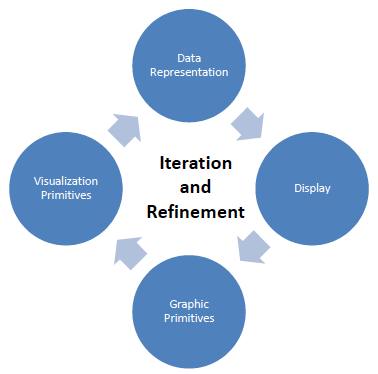
\includegraphics[width=.75\columnwidth]{figs/viz/render}
\end{beamerboxesrounded}
\end{column}
\end{columns}
\end{small}
\end{frame}


%%%%
\resetEnv

%%%%%%%%%%%%%%%%%%%%%%%%%%%%%%%%%%%%%%%%%%%%%%%%%%%%%%%%%%%%%%%%%%%
%mp Marcelo
\section{VisIt: an Overview}
\basicEnv
\frame{\sectionpage}
%%%%
 
%%%%% VisIt
%\section{VisIt}
\subsection{Generalities}
\begin{frame}
\frametitle{\href{https://wci.llnl.gov/simulation/computer-codes/visit/}{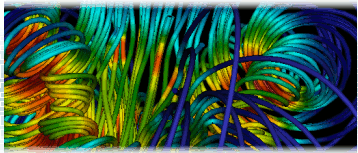
\includegraphics[height=.85cm]{figs/visit-logos/VisIt-01}} \href{https://wci.llnl.gov/simulation/computer-codes/visit/}{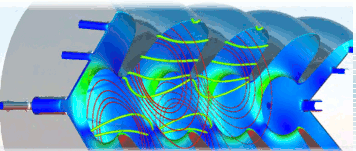
\includegraphics[height=.875cm]{figs/visit-logos/VisIt-02}} \href{https://wci.llnl.gov/simulation/computer-codes/visit/}{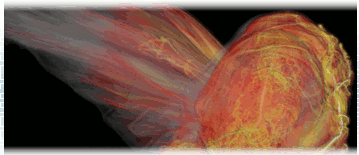
\includegraphics[height=.875cm]{figs/visit-logos/VisIt-03}} \href{https://wci.llnl.gov/simulation/computer-codes/visit/}{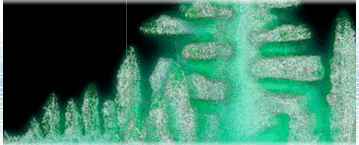
\includegraphics[height=.875cm]{figs/visit-logos/VisIt-04}} \hspace{-8.5cm}{\bf \textcolor{white}{VisIt}}}

%\vspace{-5mm}
%\hspace{-2.5mm}
%\href{https://wci.llnl.gov/simulation/computer-codes/visit}{\textcolor{DarkBlue}{\small\tt https://wci.llnl.gov/simulation/computer-codes/visit}}
%
%\hspace{-2.5mm}
%\href{http://visit.llnl.gov/}{\textcolor{DarkBlue}{\tt http://visit.llnl.gov/}}

\vspace{-3.5mm}
\begin{columns}%[T]
\begin{column}{7.65cm}
\vspace{-2mm}
\href{https://wci.llnl.gov/simulation/computer-codes/visit}{\textcolor{DarkBlue}{\small\tt https://wci.llnl.gov/simulation/computer-codes/visit}}

\href{http://visit.llnl.gov/}{\textcolor{DarkBlue}{\tt http://visit.llnl.gov/}}

\begin{small}
\begin{itemize}
        \item Developed by the \textit{DOE Advanced Simulation and Computing Initiative}, %(ASCI)
 to visualize results of terascale simulations, first release fall of 2002 -- mantained by \textit{LLNL}
        \item \textcolor{DarkRed}{v2.10.2} \href{https://wci.llnl.gov/simulation/computer-codes/visit/downloads}{available as source and binary for \textcolor{DarkBlue}{Linux/Mac/Windows}}
        \item Over 80 visualization features (contour, mesh, slice, volume, molecule, ...)
        %\item Reads over 120 different file formats (\ding{223} \href{http://www.visitusers.org/index.php?title=Detailed_list_of_file_formats_VisIt_supports}{\small detailed list of file formats})
        \item Interfaces with C++, Python, and Java
        \item Uses MPI for \textcolor{DarkBlue}{distributed-memory parallelism} on HPC clusters
\end{itemize}
\end{small}
\end{column}
\begin{column}{5cm}
	\vspace{-2mm}

        \href{https://wci.llnl.gov/simulation/computer-codes/visit/gallery}{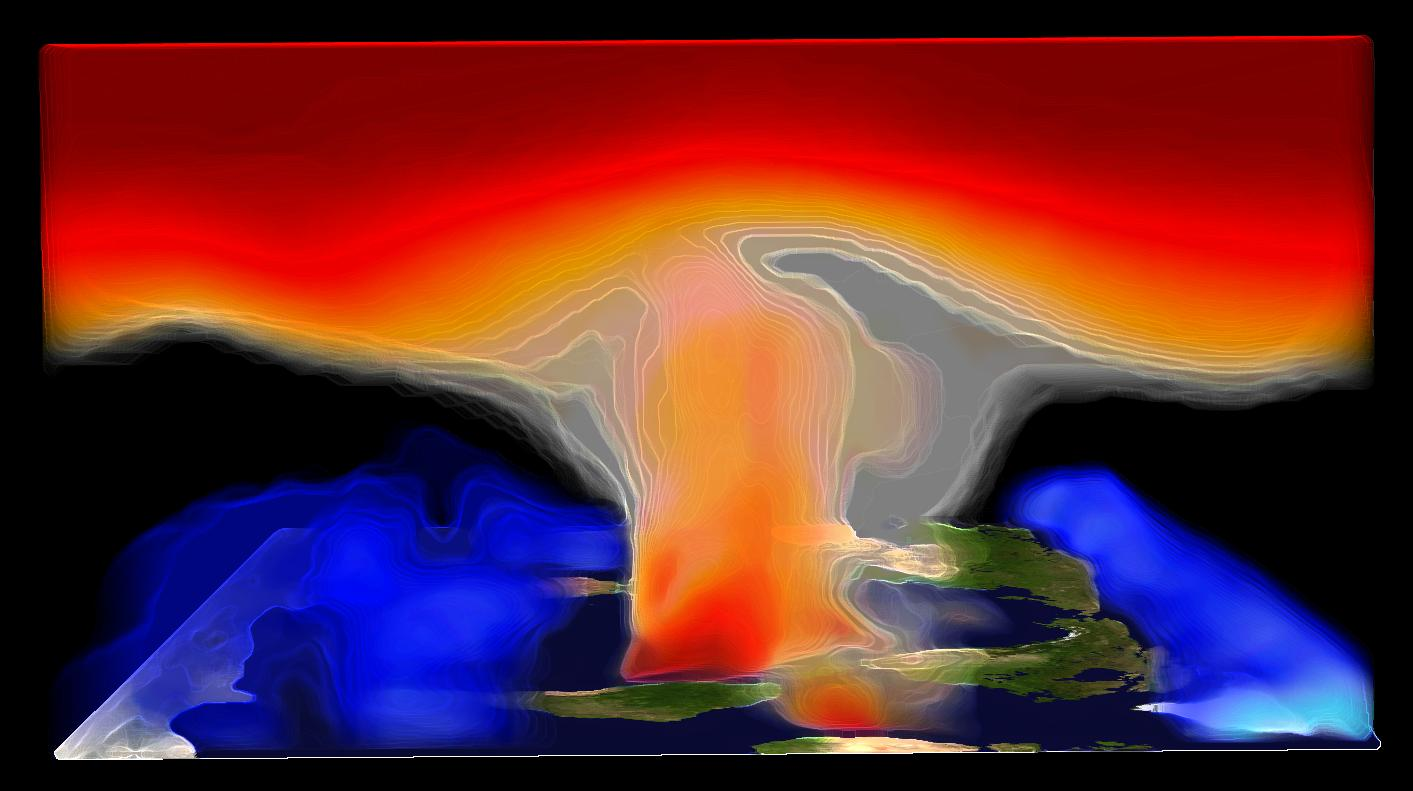
\includegraphics[width=.475\columnwidth]{figs/visit-exs/VisIt-gallery_33}}
        \href{https://wci.llnl.gov/simulation/computer-codes/visit/gallery}{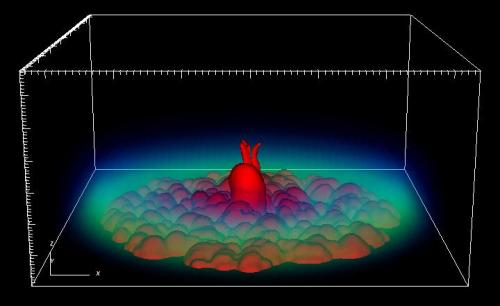
\includegraphics[width=.475\columnwidth]{figs/visit-exs/VisIt-gallery_10}}

	\vspace{-.75mm}
        \href{https://wci.llnl.gov/simulation/computer-codes/visit/gallery}{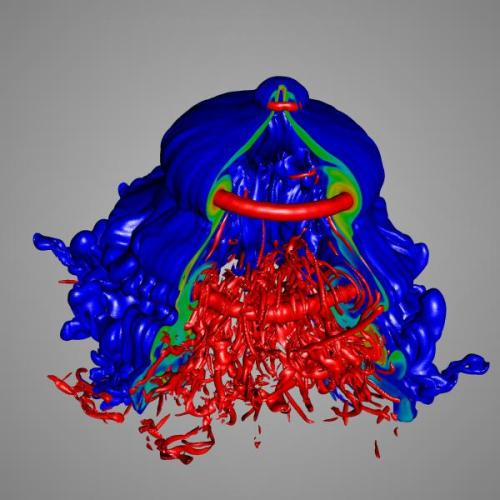
\includegraphics[width=.475\columnwidth]{figs/visit-exs/VisIt-gallery_00}}
        \href{https://wci.llnl.gov/simulation/computer-codes/visit/gallery}{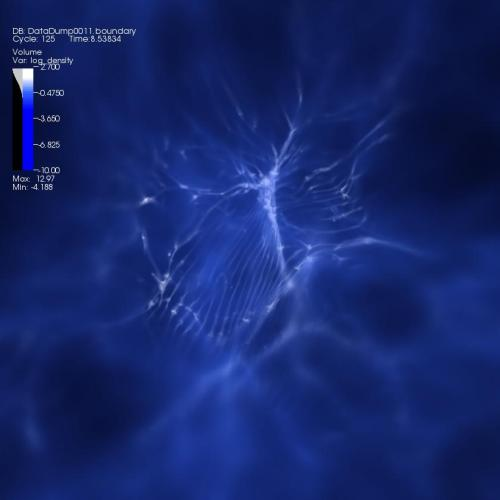
\includegraphics[width=.475\columnwidth]{figs/visit-exs/VisIt-gallery_05}}

	\vspace{-.75mm}
        \href{https://wci.llnl.gov/simulation/computer-codes/visit/gallery}{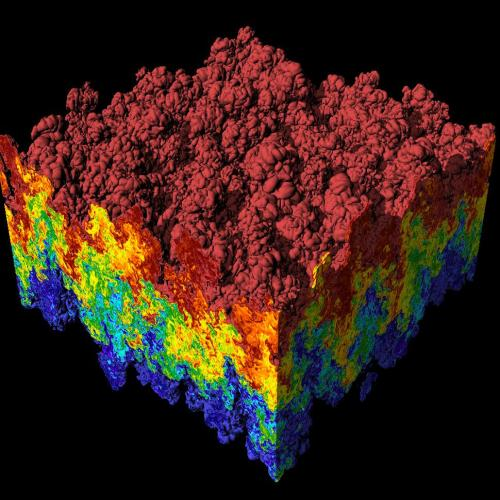
\includegraphics[width=.475\columnwidth]{figs/visit-exs/VisIt-gallery_02}}
        \href{https://wci.llnl.gov/simulation/computer-codes/visit/gallery}{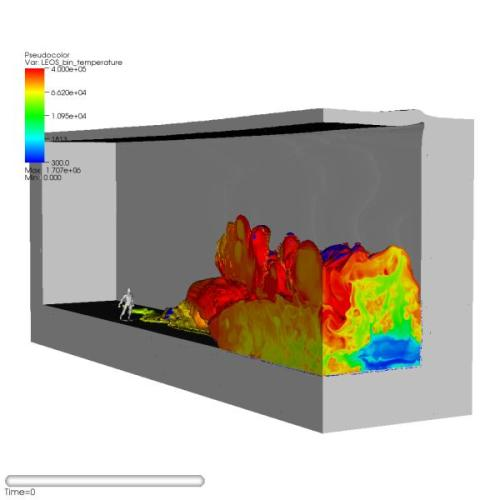
\includegraphics[width=.475\columnwidth]{figs/visit-exs/VisIt-gallery_01}}

	\vspace{-.75mm}
        \href{https://wci.llnl.gov/simulation/computer-codes/visit/gallery}{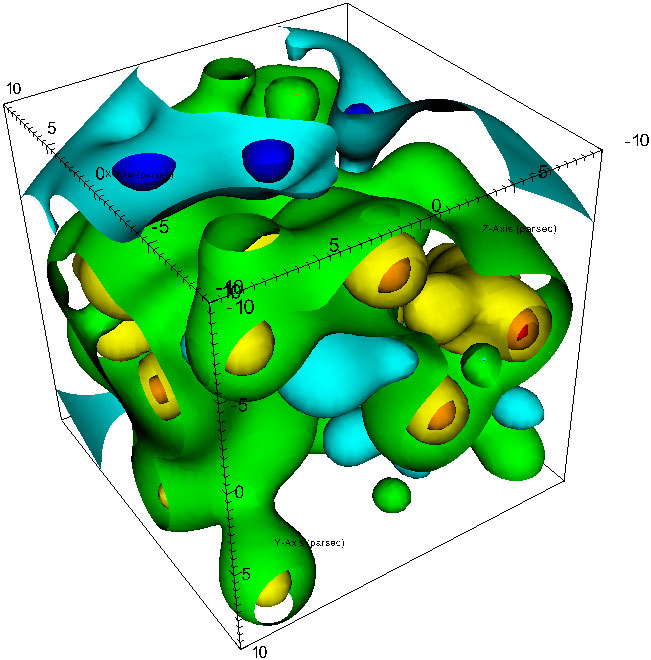
\includegraphics[width=.475\columnwidth]{figs/visit-exs/VisIt-contour1_S}}
        \href{https://wci.llnl.gov/simulation/computer-codes/visit/gallery}{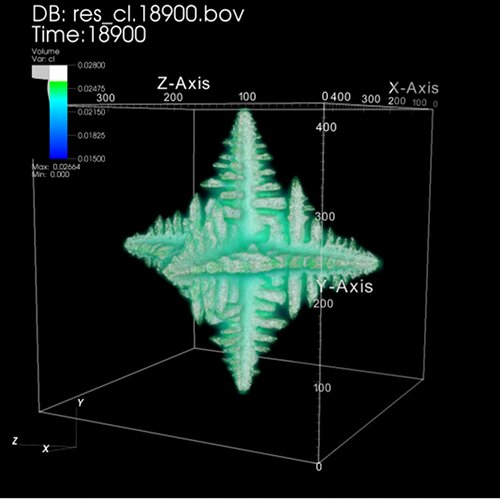
\includegraphics[width=.475\columnwidth]{figs/visit-exs/VisIt-gallery_39}}
\end{column}
\end{columns}
\end{frame}


\begin{frame}
\frametitle{\href{https://wci.llnl.gov/simulation/computer-codes/visit/}{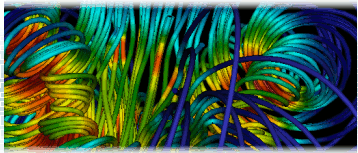
\includegraphics[height=.85cm]{figs/visit-logos/VisIt-01}} \href{https://wci.llnl.gov/simulation/computer-codes/visit/}{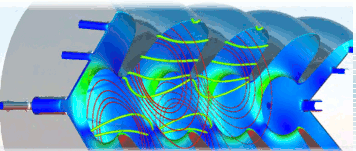
\includegraphics[height=.875cm]{figs/visit-logos/VisIt-02}} \href{https://wci.llnl.gov/simulation/computer-codes/visit/}{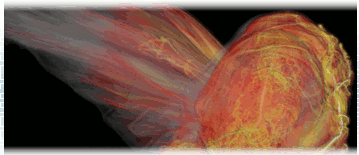
\includegraphics[height=.875cm]{figs/visit-logos/VisIt-03}} \href{https://wci.llnl.gov/simulation/computer-codes/visit/}{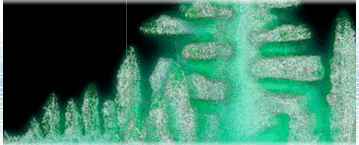
\includegraphics[height=.875cm]{figs/visit-logos/VisIt-04}} \hspace{-8.5cm}{\bf \textcolor{white}{VisIt}}}

\begin{columns}
\begin{column}{5.5cm}
\begin{itemize}
        \item can run: locally, remotelly, client/server mode
        \item interface pretty much looks the same on each platform
        \item can read over a 120 different data formats (\ding{223} \href{http://www.visitusers.org/index.php?title=Detailed_list_of_file_formats_VisIt_supports}{\small detailed list of file formats})
        \item new database plugin readers can be developed
\end{itemize}
\pause
\begin{beamerboxesrounded}[upper=block head,lower=block body,shadow=true]{\ding{232} Supported \textcolor{DarkRed}{Mesh Types} }
        \ding{231}~\textcolor{DarkBlue}{1D Curves}

        \ding{231}~\textcolor{DarkBlue}{2D/3D meshes}: Rectilinear, Curvilinear, Unstructured, Points, AMR, Molecular, CSG
\end{beamerboxesrounded}
\end{column}
\begin{column}{6.25cm}
\pause
\begin{beamerboxesrounded}[upper=block head,lower=block body,shadow=true]{\ding{232} VisIt \textcolor{DarkRed}{Architecture} }
        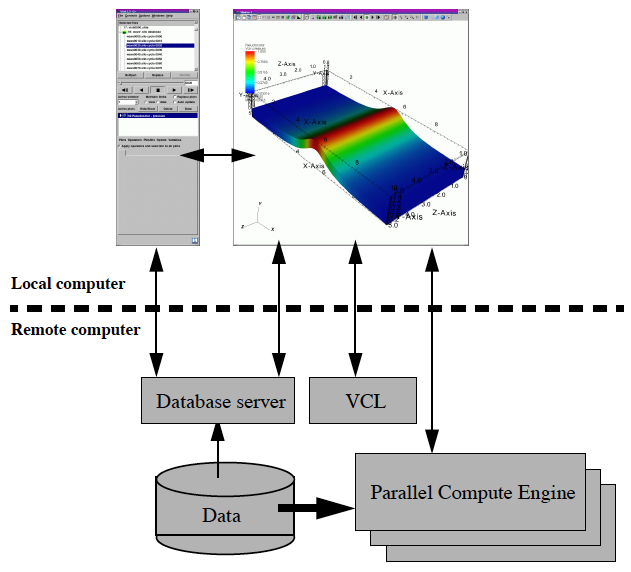
\includegraphics[width=\columnwidth]{figs/visit-guis/VisIt_arch}
\end{beamerboxesrounded}
\end{column}
\end{columns}

\end{frame}



\begin{frame}
\frametitle{\href{https://wci.llnl.gov/simulation/computer-codes/visit/}{\includegraphics[height=.85cm]{figs/visit-logos/VisIt-01}} \hspace{-.85cm}{\bf \textcolor{white}{VisIt}}: Multiple Interfaces}

\begin{columns}
\begin{column}{4.75cm}
\begin{itemize}
        \item GUI (graphical user interface)
        \item Python programming interface
        \item Java programming interface
        \item C++ programming interface
\end{itemize}
\end{column}
\begin{column}{7.25cm}
\pause
\begin{beamerboxesrounded}[upper=block head,lower=block body,shadow=true]{\ding{231} Use multiple interfaces simultaneously}
        \ding{232}~Use VisIt as an application or a library

        \ding{232}~C++, Python, Java interfaces allow other applications to control VisIt
\end{beamerboxesrounded}
\end{column}
\end{columns}
\end{frame}


\subsection{GUIs}
\begin{frame}
\frametitle{\href{https://wci.llnl.gov/simulation/computer-codes/visit/}{\href{https://wci.llnl.gov/simulation/computer-codes/visit/}{\includegraphics[height=.875cm]{figs/visit-logos/VisIt-02}} {\bf \textcolor{lightgray}{VisIt}}}: GUI}

\begin{columns}
\begin{column}{5.5cm}
\pause
\begin{beamerboxesrounded}[upper=block head,lower=block body,shadow=true]{\ding{232}  \textcolor{DarkRed}{GUI} }
        \textcolor{DarkRed}{\ding{223}} Select files to visualize

        \textcolor{DarkRed}{\ding{223}} Create and manage plots

        \textcolor{DarkRed}{\ding{223}} Set plot attributes

        \textcolor{DarkRed}{\ding{223}} Add operators

        \textcolor{DarkRed}{\ding{223}} Set look and props. for visualization
\end{beamerboxesrounded}
\pause
\begin{beamerboxesrounded}[upper=block head,lower=block body,shadow=true]{\ding{232} \textcolor{DarkBlue}{Viewer} }
        \textcolor{DarkBlue}{\ding{223}} display all of the data being visualized

        \textcolor{DarkBlue}{\ding{223}} Mouse navigation

        \textcolor{DarkBlue}{\ding{223}} up to 16 vis windows

        \textcolor{DarkBlue}{\ding{223}} Popup menu

        \textcolor{DarkBlue}{\ding{223}} Toolbars
\end{beamerboxesrounded}
\end{column}
\begin{column}{6cm}
        \centering
        \includegraphics[width=.3\columnwidth]{figs/visit-guis/VisIt_GUI}
        \includegraphics[width=.575\columnwidth]{figs/visit-guis/VisIt_viewer}

        \vspace{2mm}
        \includegraphics[width=\columnwidth]{figs/visit-guis/VisIt_windows}
\end{column}
\end{columns}
\end{frame}


\begin{frame}
\frametitle{\href{https://wci.llnl.gov/simulation/computer-codes/visit/}{\includegraphics[height=.85cm]{figs/visit-logos/VisIt-03}} \hspace{-.85cm}{\bf \textcolor{lightgray}{VisIt}}: GUIs}

\begin{columns}
\begin{column}{5cm}
\begin{beamerboxesrounded}[upper=block head,lower=block body,shadow=true]{\ding{224}  \textcolor{DarkRed}{Main window in GUI} }

        \textcolor{DarkRed}{\ding{223}} Access other important windows

        \textcolor{DarkRed}{\ding{223}} Open files

        \textcolor{DarkRed}{\ding{223}} Set animation time state

        \textcolor{DarkRed}{\ding{223}} Set active window

        \textcolor{DarkRed}{\ding{223}} Create and manage filters (pipeline)

        \textcolor{DarkRed}{\ding{223}} Displays progress from compute engine
\end{beamerboxesrounded}

\pause
\vspace{1mm}
\begin{beamerboxesrounded}[upper=block head,lower=block body,shadow=true]{\ding{231} Really useful ones}
        \hspace{1.25mm}
        \textcolor{DarkBlue}{\ding{232} Apply to... } check-boxes
\end{beamerboxesrounded}
\end{column}
\begin{column}{6cm}
        \centering
        \includegraphics[clip=true,trim=0 0 17cm 0, width=.85\columnwidth]{figs/visit-guis/VisIt_windows}
\end{column}
\end{columns}
\end{frame}


\begin{frame}
\frametitle{\href{https://wci.llnl.gov/simulation/computer-codes/visit/}{\includegraphics[height=.85cm]{figs/visit-logos/VisIt-04}} \hspace{-.85cm}{\bf \textcolor{white}{VisIt}}: GUIs}

\vspace{-3mm}
\begin{columns}
\begin{column}{5cm}
\begin{beamerboxesrounded}[upper=block head,lower=block body,shadow=true]{\ding{224}  \textcolor{DarkBlue}{Main Menu} }

        \textcolor{DarkBlue}{\ding{223}} \framebox{File}

        \textcolor{DarkBlue}{\ding{223}} \framebox{Controls}

        \textcolor{DarkBlue}{\ding{223}} \framebox{Options}

        \textcolor{DarkBlue}{\ding{223}} \framebox{Windows}

        \textcolor{DarkBlue}{\ding{223}} \framebox{Plot Attributes}

        \textcolor{DarkBlue}{\ding{223}} \framebox{Operator Attributes}

        \textcolor{DarkBlue}{\ding{223}} \framebox{Help}
\end{beamerboxesrounded}
\end{column}
\begin{column}{6cm}
        \centering
        \includegraphics[clip=true,trim=0 0 17cm 0, width=.85\columnwidth]{figs/visit-guis/VisIt_windows}
\end{column}
\end{columns}

\begin{beamerboxesrounded}[upper=block head,lower=block body,shadow=true]{\ding{224}  \textcolor{DarkBlue}{Visualization Toolbar} }
        \centering
        \includegraphics[width=.85\columnwidth]{figs/visit-guis/VisIt_toolbar}
\end{beamerboxesrounded}
\end{frame}



\subsection{Core Abstractions}
\begin{frame}
\frametitle{VisIt's Core Abstractions}
\begin{columns}
\begin{column}{5cm}
	\begin{beamerboxesrounded}{\textcolor{orange}{*} Databases}
		access the \textbf{data}
	\end{beamerboxesrounded}

	\begin{beamerboxesrounded}{\textcolor{orange}{*} Plots}
		\textbf{visualize} (render) the data
	\end{beamerboxesrounded}

	\begin{beamerboxesrounded}{\textcolor{orange}{*} Operators}
		\textbf{process} --manipulate-- the data
	\end{beamerboxesrounded}

	\begin{beamerboxesrounded}{\textcolor{orange}{*} Expressions}
		derive quantities
	\end{beamerboxesrounded}

	\begin{beamerboxesrounded}{\textcolor{orange}{*} Queries}
		obtain quantitative info
	\end{beamerboxesrounded}
\end{column}
\begin{column}{5cm}
\end{column}
\end{columns}
\end{frame}



\subsection{Viz Pipeline}
\begin{frame}
\frametitle{\href{https://wci.llnl.gov/simulation/computer-codes/visit/}{\includegraphics[height=.85cm]{figs/visit-logos/VisIt-01}} \hspace{-.85cm}{\bf \textcolor{lightgray}{VisIt}}: Visualization Pipeline}

\begin{columns}
\begin{column}{5cm}
\begin{beamerboxesrounded}[upper=block head,lower=block body,shadow=true]{}
\begin{enumerate}
        \item Open database (or file)
        \item Create a plot
        \item Set plot attributes
        \item Apply operators to plot to modify data
        \item Set operator attributes
        \item Compute engine generates plot
        \item Plot displayed in vis window
        \item iterate//repeat...
\end{enumerate}
\end{beamerboxesrounded}
\end{column}
\begin{column}{6cm}
        \centering
        \includegraphics[width=.85\columnwidth]{figs/viz/viz-pipeline4}
\end{column}
\end{columns}

\end{frame}


 % includes the following topics:
 % - introduction and VisIt's GUI overview
%%%%
\resetEnv

%%%%%%%%%%%%%%%%%%%%%%%%%%%%%%%%%%%%%%%%%%%%%%%%%%%%%%%%%%%%%%%%%%%
%mp Marcelo and some contribution from Alex
\section{VisIt: Basic Visualization Tools}
\basicEnv
\frame{\sectionpage}
%%%%
 
%\subsection{A guided example...}
\subsection{Reading data...}
\begin{frame}
\frametitle{\href{https://wci.llnl.gov/simulation/computer-codes/visit/}{\includegraphics[height=.85cm]{figs/visit-logos/VisIt-02}} \hspace{-.85cm}{\bf \textcolor{lightgray}{VisIt}}: Import Data}

\begin{columns}
\begin{column}{6.25cm}
        \textcolor{DarkRed}{*} Importing datasets

        \textcolor{DarkBlue}{$\blacktriangleright$}
        \framebox{File} $\rightarrow$ \framebox{\bf Open file...}

        \hspace{2mm} $\mapsto$ choose data file {\small (eg. ``\textcolor{gray}{noise.silo}'')}

        \pause
        \vspace{2mm}
        \begin{beamerboxesrounded}[upper=block head,lower=block body,shadow=true]{\ding{231} Become available}
                \hspace{2mm}
                \ding{232} \textcolor{DarkBlue}{Active source}: ``\textcolor{gray}{noise.silo}''

                \hspace{2mm}
                \ding{232} \textcolor{DarkBlue}{Add button}
        \end{beamerboxesrounded}

        \pause
        \vspace{2mm}
        \textcolor{DarkBlue}{$\blacktriangleright$}
        \framebox{File} $\rightarrow$ \framebox{\bf File information...}
\end{column}
\begin{column}{5.5cm}
        \textcolor{DarkRed}{*} Restoring a previous session

        \vspace{2.5mm}
        \textcolor{DarkBlue}{$\blacktriangleright$}
        \framebox{File} $\rightarrow$ \framebox{\bf Restore session...}
        \\
        loads the previous state of the given session (\textbf{that needs to be specifically saved})

        \vspace{3.5mm}
        \textcolor{DarkBlue}{$\blacktriangleright$}
        \framebox{File} $\rightarrow$ \framebox{\bf Restore session w/sources...}
        \\
        extremely useful for re-identifiying datasets that could have been moved or renamed
        %\centering
        %\includegraphics[width=.85\columnwidth]{figs/}
\end{column}
\end{columns}
\pause
\vspace{2mm}
\begin{beamerboxesrounded}[upper=block head,lower=block body,shadow=true]{}
Be aware, that VisIt, by default won't save your work (session) nor ask you when you try to exit the program!
\end{beamerboxesrounded}
\end{frame}




\subsection{Contours: Iso-Surfaces \& Iso-Curves}
\begin{frame}
\frametitle{\href{https://wci.llnl.gov/simulation/computer-codes/visit/}{\includegraphics[height=.85cm]{figs/visit-logos/VisIt-03}} \hspace{-.85cm}{\bf \textcolor{lightgray}{VisIt}}: Contours}

\begin{columns}
\begin{column}{5cm}
        \textcolor{DarkBlue}{$\blacktriangleright$}
        \framebox{Add$_\blacktriangledown$} $\rightarrow$ \framebox{Contours}

        \hspace{5.5mm}
        $\leadsto$ \framebox{\textcolor{DarkGreen}{\it hardyglobal}}

        \hspace{5.5mm}
        $\rightarrow$ \framebox{\textcolor{DarkBlue}{Draw}}

        \centering
        \includegraphics[width=\columnwidth]{figs/visit-pract/VisIt_contour}
\end{column}
\begin{column}{6.5cm}
        \centering
        \includegraphics[width=\columnwidth]{figs/visit-pract/VisIt_contour1a}
\end{column}
\end{columns}
\end{frame}


\begin{frame}
\frametitle{\href{https://wci.llnl.gov/simulation/computer-codes/visit/}{\includegraphics[height=.85cm]{figs/visit-logos/VisIt-04}} \hspace{-.85cm}{\bf \textcolor{lightgray}{VisIt}}: Contours}

\begin{columns}
\begin{column}{6cm}
        \textcolor{DarkBlue}{\ding{224}}
        double-click on \textcolor{DarkGreen}{Contour-hardyglobal}

        \pause
        \textcolor{DarkBlue}{\ding{224}}
        under \textcolor{DarkBlue}{Select by}, choose \framebox{\textcolor{DarkGreen}{N levels}} = \textcolor{blue}{5} \Enter

        \pause
        \textcolor{DarkBlue}{\ding{224}}
        Change \textcolor{DarkBlue}{opacity levels}, eg: 100\%, 60\%, 60\%, 48\%, 24\%

        \centering
        \includegraphics[width=.65\columnwidth]{figs/visit-pract/VisIt_contour-props}
\end{column}
\begin{column}{5.5cm}
        %\pause
        \textcolor{DarkBlue}{\ding{224}}
        \framebox{Apply}
        \&
        \framebox{Dismiss}

        \vspace{3mm}
        %\centering
        \includegraphics[width=\columnwidth]{figs/visit-pract/VisIt_contour1b}

        \pause
        \vspace{3mm}
        %\left
        \textcolor{DarkBlue}{\ding{224}}
        \framebox{Hide/Show}
        or
        \framebox{Delete}
\end{column}
\end{columns}
\end{frame}

\begin{frame}
\frametitle{\href{https://wci.llnl.gov/simulation/computer-codes/visit/}{\includegraphics[height=.85cm]{figs/visit-logos/VisIt-01}} \hspace{-.85cm}{\bf \textcolor{lightgray}{VisIt}}: PseudoColor \& IsoSurfaces}
\vspace{-1.85mm}
\begin{columns}
\begin{column}{6cm}
        \textcolor{DarkBlue}{\ding{224}}
        \framebox{Add$_\blacktriangledown$} $\rightarrow$ \framebox{\textcolor{DarkRed}{\bf Pseudocolor}}

        \hspace{5.5mm}
        $\leadsto$ \framebox{\textcolor{DarkGreen}{\it hardyglobal}}

        \hspace{5.5mm}
        $\rightarrow$ \framebox{\textcolor{DarkBlue}{Draw}}

        \centering
        \includegraphics[width=\columnwidth]{figs/visit-pract/VisIt_pseudocolor}
\end{column}
\begin{column}{6cm}
        \pause
        \textcolor{DarkBlue}{\ding{224}}
        \framebox{Operators$_\blacktriangledown$}
                $\rightarrow$ \framebox{\bf Slicing}

        \hspace{5.5mm}
        $\rightarrow$ \framebox{\textcolor{DarkRed}{\bf Isosurface}}

        \hspace{5.5mm}
        $\rightarrow$ \framebox{\textcolor{DarkBlue}{Draw}}

        \centering
        \includegraphics[width=\columnwidth]{figs/visit-pract/VisIt_pseudocolor-isosurf}
\end{column}
\end{columns}

\pause
\vspace{2mm}
\textcolor{DarkBlue}{\ding{224}}
        click $\blacktriangleright$ to expand, double click on [\textcolor{DarkBlue}{Isosurface}]

\hspace{4mm}
\textcolor{DarkBlue}{\ding{223}}
under \textcolor{DarkBlue}{Select by}, choose \framebox{\textcolor{DarkGreen}{Percent (s)}} = \textcolor{blue}{50} \Enter \& \framebox{Dismiss}


\pause
\vspace{2mm}
\textcolor{DarkBlue}{\ding{224}}
        change the \textcolor{DarkRed}{opacity} of [\textcolor{DarkBlue}{Pseudocolor}]
\end{frame}


\begin{frame}
\frametitle{\href{https://wci.llnl.gov/simulation/computer-codes/visit/}{\includegraphics[height=.85cm]{figs/visit-logos/VisIt-02}} \hspace{-.85cm}{\bf \textcolor{lightgray}{VisIt}}: PseudoColor \& IsoSurfaces}
\vspace{-1.5mm}
\begin{columns}%[T]
\begin{column}{9cm}
        \centering
        \includegraphics[width=\columnwidth]{figs/visit-pract/VisIt_pseudocolor-isosurf_2}
\end{column}
\begin{column}{3cm}
        \pause
        \textcolor{DarkBlue}{\ding{224}}
        unselect the [\textcolor{DarkBlue}{Apply ...}] check-boxes

        \vspace{2mm}
        \textcolor{DarkBlue}{\ding{224}} add 1 more
                \textcolor{DarkRed}{Pseudocolor}
                +\textcolor{DarkRed}{\bf Isosurface},
        \\
        %\hspace{1.5mm}
        w/\textcolor{DarkBlue}{Percent(s)=80}
        \& adjust its
        \textcolor{DarkBlue}{opacity}
\end{column}
\end{columns}

\pause
\vspace{2mm}
\textcolor{DarkBlue}{\ding{224}}
        \textcolor{blue}{clipping} \ding{223} select/check the [\textcolor{DarkBlue}{Apply...}] boxes

%\vspace{1mm}
\textcolor{DarkBlue}{\ding{224}}
        \framebox{Operators$_\blacktriangledown$}
                $\rightarrow$ \framebox{\bf Selection}
        %\hspace{5.5mm}
        $\rightarrow$ \framebox{\textcolor{DarkRed}{\bf Clip}}

        \hspace{5mm}
        \ding{223} choose \textcolor{DarkBlue}{combinations of $\ne$ planes} to modify the $\ll$clip$\gg$
\end{frame}















\begin{frame}
\frametitle{\href{https://wci.llnl.gov/simulation/computer-codes/visit/}{\includegraphics[height=.85cm]{figs/visit-logos/VisIt-03}} \hspace{-.85cm}{\bf \textcolor{lightgray}{VisIt}}: General Remarks}

\begin{beamerboxesrounded}[upper=block head,lower=block body,shadow=true]{}
        \textcolor{DarkBlue}{\ding{231}} operators/plots can be removed
                \framebox{\textcolor{DarkBlue}{\bf Delete}}
                --or--
                hidden \framebox{\textcolor{DarkBlue}{\bf Hide/Show}}

        \textcolor{DarkBlue}{\ding{231}} save your work {\bf frequently}:
                \framebox{File} $\rightarrow$ \framebox{\textcolor{DarkBlue}{\bf Save session...}}
\end{beamerboxesrounded}

\pause
\vspace{3mm}
\begin{beamerboxesrounded}[upper=block head,lower=block body,shadow=true]{Hands-on...}%Assignment ii}
        \textcolor{DarkRed}{\ding{231}} try loading some of the datasets we used with ParaView [{\small \textcolor{gray}{\tt headsq.vtk}, \textcolor{gray}{\tt testRectilinearGrid.vtk}, \textcolor{gray}{\tt disk\_out\_ref.ex2}, ...}] --or-- your own data!!!

        \textcolor{DarkRed}{\ding{231}} and compare how easy/possible or not, is to obtain similar results, let's say, to ParaView for instance...

        \textcolor{DarkRed}{\ding{231}} also which one, results more intuitive, elegant, useful for you and your research
\end{beamerboxesrounded}
\end{frame}


 % includes the following topics:
 % - accessing data and managing files
 % - working with plots
 % - working with operators
 % - interactive tools
 % - plots, selections, exporting
%%%%
 \handsonEnv
%%%
\begin{frame}
\frametitle{\href{https://wci.llnl.gov/simulation/computer-codes/visit/}{\includegraphics[height=.85cm]{figs/visit-logos/VisIt-03}} \hspace{-.85cm}{\bf \textcolor{lightgray}{VisIt}}: Intermesso i}

\begin{beamerboxesrounded}[upper=block head,lower=block body,shadow=true]{\bf Hands-on...}%Assignment ii}
%        \textcolor{DarkRed}{\ding{231}} try loading some of the datasets we used with ParaView [{\small \textcolor{gray}{\tt headsq.vtk}, \textcolor{gray}{\tt testRectilinearGrid.vtk}, \textcolor{gray}{\tt disk\_out\_ref.ex2}, ...}] --or-- your own data!!!
        \textcolor{DarkGreen}{\ding{231}} Load some of the other datasets: 
                [eg. {\small \textcolor{gray}{\tt headsq.vtk}, \textcolor{gray}{\tt testRectilinearGrid.vtk}, \textcolor{gray}{\tt disk\_out\_ref.ex2}, ...}]
                --or-- \textit{your own data}!!!

        \pause
        \textcolor{DarkGreen}{\ding{231}} Try to explore the data and visualize it, using some of the tools we have discussed

	\pause
        \textcolor{DarkGreen}{\ding{231}} If you have used other visualization packages, compare how easy and 
                whether it is possible or not, to obtain similar results, let's say, with ParaView or VAPOR for instance...

        \textcolor{DarkGreen}{\ding{231}} also which one, results more intuitive, elegant, useful for you and your research
\end{beamerboxesrounded}

\pause
\vspace{2mm}
\begin{columns}
\begin{column}{3cm}
	\includegraphics[width=.9\columnwidth]{figs/visit-handson/testRectilinearGrid}
\end{column}
\begin{column}{3cm}
	\includegraphics[width=.9\columnwidth]{figs/visit-handson/headsq}
\end{column}
\begin{column}{3cm}
	\includegraphics[width=.9\columnwidth]{figs/visit-handson/headsq_cut}
\end{column}
\end{columns}
\end{frame}

\begin{frame}
	\includegraphics[width=.55\columnwidth]{figs/visit-handson/testRectilinearGrid_gui}

	\includegraphics[width=.55\columnwidth]{figs/visit-handson/headsq_gui}
	\includegraphics[width=.55\columnwidth]{figs/visit-handson/headsq-cut_gui}
\end{frame}
%%%
\resetEnv
\basicEnv

%%%%
\resetEnv

%%%%%%%%%%%%%%%%%%%%%%%%%%%%%%%%%%%%%%%%%%%%%%%%%%%%%%%%%%%%%%%%%%%%
%ar Alex
\section{Quantitative analysis with VisIt}
\normalEnv
\frame{\sectionpage}
%%%%
 \begin{comment}
  http://www.vtk.org/download - Download VTK textbook examples and data - PineRoot.tgz
  http://www.vtk.org/files/release/7.0/VTKLargeData-7.0.0.zip


  Cross-mesh field evaluation (CMFE) and database comparison
  \url{http://www.visitusers.org/index.php?title=Cmfe_overview}
  \url{http://www.visitusers.org/index.php?title=Cross_Mesh_Field_Evaluation}
  The CMFE expressions evaluate a field from a donor mesh onto a target mesh to form a new field.

  Data level comparison wizard
    \url{http://www.visitusers.org/index.php?title=VisIt-tutorial-comparison}

    
\end{comment}

\begin{frame}{Quantitative analysis}{}
  \begin{itemize}\setlength{\itemsep}{3mm}
    % - p.233
  \item Expressions (similar to the Calculator filter in ParaView)
  \item Pick: zone/node, spreadsheet, time curves
  \item Lineout
  \item Queries
  \item Time sliders and database correlations
  \end{itemize}
\end{frame}

\begin{frame}{Expressions}
  \begin{itemize}\setlength{\itemsep}{3mm}
  \item Create new derived variables from existing ones
  \item Mathematical expressions can operate on scalars, vectors, tensors
  \item {\bf Option 1}: use Standar Editor to select existing functions and expressions \\\ding{48}
    similar to the Calculator filter in ParaView
  \item {\bf Option 2}: use Python Expression Editor - this is an advanced option for working
    with VTK objects; we'll cover it in the Scripting session \\\ding{48} similar to the Programmable
    filter in ParaView
  \end{itemize}
\end{frame}

\begin{frame}{Expressions}
  \begin{beamerboxesrounded}[upper=block head,lower=block body,shadow=true]{}
    \begin{itemize}\setlength{\itemsep}{0mm}
    \item Load sineEnvelope.nc, visualize density with Pseudocolor
    \item Controls \ra Expressions \ra New, set name = densitySquared, type = Scalar Mesh Variable,
      definition = density$\hat{\,\,\,}$2, click Apply
    \item Now in the list of variables switch to densitySquared
    \end{itemize}
  \end{beamerboxesrounded}
  \medskip
  \pause
  \begin{beamerboxesrounded}[upper=block head,lower=block body,shadow=true]{}
    \begin{itemize}\setlength{\itemsep}{0mm}
    \item Controls \ra Expressions \ra New, set name = densityGradient, type = VectorMeshVariable,
      definition = gradient(density)
    \item You can use the dropdown menus to accelerate typing (gradient
      will be found in Insert Function \ra Miscellaneous)
    \item Add a vector plot to show densityGradient, picking ``Uniformly located troughout the mesh'',
      displaying 5000 vectors, overlaying them onto a semi-transparent Pseudocolor plot of density
    \end{itemize}
  \end{beamerboxesrounded}
  \medskip
  \pause
  \begin{beamerboxesrounded}[upper=block head,lower=block body,shadow=true]{}
    \begin{itemize}\setlength{\itemsep}{0mm}
    \item Controls \ra Expressions \ra New, set name = truncatedDensity, type=VectorMeshVariable,
      definition=max(1,density)
    \item Now in the list of variables switch to truncatedDensity
    \end{itemize}
  \end{beamerboxesrounded}
\end{frame}

\begin{frame}{Pick}
  \begin{itemize}\setlength{\itemsep}{3mm}
  \item Interactively pick values inside the visualization window
  \item Load sineEnvelope.nc, visualize density with Pseudocolor, apply Operators \ra Selection \ra Clip,
    click Draw
  \item Data here is defined on nodes, not zones
    \pause
  \item Right click on the vis, select Mode \ra Zone Pick (or use a mode button in the vis window
    toolbar), and click anywhere on the vis -- it'll display 8 nodes forming the zone, and their variable
    values
    \begin{itemize}\setlength{\itemsep}{0mm}
    \item each pick point leaves a marker that you can look up in the Pick window
    \item the Pick window displays information in tabs arranged by a point
    \end{itemize}
    \pause
  \item Similarly, Mode \ra Node Pick will display a single node, its variable, and its 8 ``incident''
    zones
  \end{itemize}
\end{frame}

\begin{frame}{Pick}
  \begin{itemize}\setlength{\itemsep}{3mm}
  \item Selecting Mode \ra Spreadsheet Pick shows a spreadsheet view of one of the dataset variables
    highlighting the picked node
    \pause
  \item Mode \ra Navigate will take you back to default interaction
    \pause
  \item Try loading a time-dependent dataset, e.g., \texttt{2d0**.vtk}
    \begin{itemize}\setlength{\itemsep}{0mm}
    \item a time slider will become active
    \item depending on the data use either Zone Pick or Node Pick
    \item inside the Pick window select ``Create time curve with next pick''
    \end{itemize}
  \end{itemize}
\end{frame}

\begin{frame}{Pick: lineout}
  \begin{itemize}\setlength{\itemsep}{2mm}
  \item Extracts 1D curves from 2D data (does not seem to work on 3D datasets)
  \item Load a 2D dataset or apply Operators \ra Slicing \ra Slice to a 3D dataset
  \item Select Mode \ra Lineout and draw a line -- the profile will be plotted in a new window
  \end{itemize}
\end{frame}

\begin{frame}{Queries}
  \begin{itemize}\setlength{\itemsep}{2mm}
  \item Controls \ra Query
  \item {\bf Option 1}: use Standard Queries
    \begin{itemize}\setlength{\itemsep}{0mm}
    \item very useful: Memory Usage
    \item quick ways to probe data: MinMax, NumNodes, NumZones, Average Value, Volume
    \item Lineout and Pick are also queries (this time enter selection manually)
    \item certain queries provide a Time Curve button that calculates the query on each time step and
      creates a curve
    \end{itemize}
  \item {\bf Option 2}: use Python Query Editor for custom queries -- we'll cover it in the Scripting
    session
  \end{itemize}
\end{frame}

\begin{frame}{More on time sliders}
  \begin{itemize}\setlength{\itemsep}{2mm}
  \item Controls \ra Database correlations
  \end{itemize}
\end{frame}

 % includes the following topics:
 % - expressions
 % - pick: zone/node, spreadsheet
 % - lineout
 % - queries
 % - time sliders
 % - database correlations
%%%%
\resetEnv

%%%%%%%%%%%%%%%%%%%%%%%%%%%%%%%%%%%%%%%%%%%%%%%%%%%%%%%%%%%%%%%%%%%%
%mp Marcelo
\section{VisIt: Proffesional Quality Plots \& Movies Generation}
\normEnv
\frame{\sectionpage}
%%%%
 
\subsection{Professional Quality Plots}
\begin{frame}
\frametitle{Professional Quality Plots}
\begin{columns}
\begin{column}{4cm}
\begin{itemize}
	\item Annotations
	\item Colors
	\item Lighting
	\item Views
\end{itemize}
\end{column}
\begin{column}{6cm}
	\includegraphics[width=\columnwidth]{figs/visit-guis/visit_ctrls}
\end{column}
\end{columns}
\end{frame}

\subsubsection{Annotations}
\begin{frame}
\frametitle{Annotations}
\begin{columns}
\begin{column}{5cm}
\begin{block}{Annotations}
\begin{itemize}
	\item objects in the viz-window
		that convey infromation about the plots
	\item make clear what is being visualized and make
		the visualization appear more polished
\end{itemize}
\end{block}
\end{column}
\begin{column}{5cm}
\begin{block}{Types of Annotations}
\begin{itemize}
        \item Database name
        \item User name
	\item plot legends
	\item plot axes and labels (2d \& 3d)
	\item 3d triad
	\item 2d, 3d text
	\item time slider
	\item images
	\item line and arrows
\end{itemize}
\end{block}
\end{column}
\end{columns}
\end{frame}


\begin{frame}
\frametitle{Annotation Window}
\begin{columns}
\begin{column}{5cm}
\begin{itemize}
        \item General annotations
        \item 2D axes settings
        \item 3D axes settings
        \item Array axis settings
	\item Color and Backgrounds
	\item Objects (legend, timr slider, ...)
\end{itemize}
\end{column}
\begin{column}{5cm}
        \includegraphics[width=\columnwidth]{figs/visit-guis/visit_annot}
\end{column}
\end{columns}
\end{frame}


\begin{frame}
\frametitle{2D \& 3D Annotations}
\begin{columns}
\begin{column}{5.75cm}
	\includegraphics[width=\columnwidth]{figs/visit-guis/visit_2d-objects}

	\vspace{2mm}
	\textcolor{DarkBlue}{\ding{224}}
        \framebox{Controls} $\rightarrow$ \framebox{\bf Annotation...}
		\ding{232}[\textcolor{DarkBlue}{\bf "2D" tab}]
\end{column}
\begin{column}{5.25cm}
        \includegraphics[width=\columnwidth]{figs/visit-guis/visit_3d-objects}

	\vspace{2mm}
        \textcolor{DarkBlue}{\ding{224}}
        \framebox{Controls} $\rightarrow$ \framebox{\bf Annotation...}
		\ding{232}[\textcolor{DarkBlue}{\bf "3D" tab}]
\end{column}
\end{columns}
\end{frame}


\begin{frame}
\frametitle{Colors and Backgrounds}
\begin{columns}
\begin{column}{6cm}
        \textcolor{DarkBlue}{\ding{224}}
        \framebox{Controls} $\rightarrow$ \framebox{\bf Annotation...}

	\hspace{5mm}
	\ding{232}[\textcolor{DarkBlue}{\bf "Colors" tab}]

	\begin{itemize}
		\item set background/foreground
		\item Backgroun styles:
		\begin{itemize}
		\item solid
		\item gradient
		\item image (flat image)
		\item image sphere (warped image, that rotates witht the view)
		\item number of repetitions
		\end{itemize}
	\end{itemize}

	\includegraphics[width=\columnwidth]{figs/visit-pract/VisIt_backgrounds}
\end{column}
\begin{column}{4.75cm}
        \includegraphics[width=\columnwidth]{figs/visit-guis/visit_annot-colors}
\end{column}
\end{columns}
\end{frame}


\begin{frame}
\frametitle{Annotation Objects}
\begin{columns}
\begin{column}{5.5cm}
        \textcolor{DarkBlue}{\ding{224}}
        \framebox{Controls} $\rightarrow$ \framebox{\bf Annotation...}

        \hspace{5mm}
        \ding{232}[\textcolor{DarkBlue}{\bf "Objects" tab}]

        \begin{itemize}
                \item 2D/3D Text
		\item 2D/3D Lines
                \item Time Slider
                %\begin{itemize}
                %\item shows progress through an animation
                %\end{itemize}
		\item Image
        \end{itemize}

	\centering
	\vspace{-2mm}
	\includegraphics[width=.855\columnwidth]{figs/visit-pract/VisIt_timeSlider}
\end{column}
\begin{column}{4.5cm}
        \includegraphics[width=\columnwidth]{figs/visit-guis/visit_annot-objects}
\end{column}
\end{columns}
\end{frame}


\subsubsection{Lighting}
\begin{frame}
\frametitle{Lighting}
\vspace{-5mm}
\begin{columns}[T]
\begin{column}{6cm}
\begin{itemize}
        \item Lighting affects the brightness of plots
        \item 3D visualizations may require multiple \textit{light sources}
        \item VisIt allows up to 8 light sources
        \item Each light source can be positioned and colored
\end{itemize}

	\pause
        \textcolor{DarkBlue}{\ding{224}}
        \framebox{Controls} $\rightarrow$ \framebox{\bf Lighting...}

	\pause
        \vspace{-1.5mm}
	\begin{block}{}
	\begin{itemize}
	\item ~[Edit]: configure light sources
	\item ~[Preview]: all sources are visible
	\end{itemize}

	\centering
	\vspace{-2mm}
	\includegraphics[width=.65\columnwidth]{figs/visit-guis/visit_lighting}
	\end{block}
\end{column}
\begin{column}{5.5cm}
	\pause
        \includegraphics[width=.85\columnwidth]{figs/visit-guis/visit_lighting2}

	\vspace{-2mm}
	\begin{block}{}
	\begin{itemize}
		\item only the active light can be modified
		\item once a light has been selected, you can change its props.
		\item Types of lights: Ambient, Camera, Object Light
		\item Position, Color, Brightness
	\end{itemize}
	\end{block}
\end{column}
\end{columns}
\end{frame}


\subsubsection{Views}
\begin{frame}
\frametitle{View}
\vspace{-2.5mm}
\begin{columns}
\begin{column}{12.5cm}
\begin{itemize}
        \item the ``view'' can be set \textit{interactively} in the viz-window (click and drag, ...)
        \item or using a ``View Window'', to specify exactly the configuration view
\end{itemize}
\end{column}
\end{columns}

        \pause
        \textcolor{DarkBlue}{\ding{224}}
        \framebox{Controls} $\rightarrow$ \framebox{\bf View...}

\vspace{-1mm}
\begin{columns}[T]
\begin{column}{3cm}
        \includegraphics[width=.9\columnwidth]{figs/visit-guis/visit_view2d}
\end{column}
\begin{column}{3cm}
	\includegraphics[width=.9\columnwidth]{figs/visit-guis/visit_view3d}
\end{column}
\begin{column}{3cm}
	\includegraphics[width=.9\columnwidth]{figs/visit-guis/visit_viewAdv}
\end{column}
\end{columns}

\begin{itemize}
	\item ``\textbf{Locked view}'': when the view changes in any locked window, all other locked window readjust to it
	\item accessible from the [Advanced] tab or ``Lock View'' tool on the viz-window
\end{itemize}

\end{frame}


\subsubsection{Images/Figures Generation: Plotting}
\begin{frame}
\frametitle{Generating ``hardcopies'', aka plotting images and figures}
\vspace{-2.5mm}
\begin{columns}
\begin{column}{5.75cm}
        \begin{block}{Generating Hardcopies: Figures}
        \begin{enumerate}

	\item
        \textcolor{DarkBlue}{\ding{224}}
        \framebox{File} $\rightarrow$ \framebox{\bf Set Save option...}

	Allows you to control the properties of the image: file type, resolution, naming convention, etc...

	\item
	\textcolor{DarkBlue}{\ding{224}}
        \framebox{File} $\rightarrow$ \framebox{\bf Save window}

	Generates the image/file of the currently displayed window.

	\end{enumerate}
	\end{block}
\end{column}
\begin{column}{5cm}
	\includegraphics[width=\columnwidth]{figs/visit-guis/visit_saveOpts}
\end{column}
\end{columns}

\end{frame}





\subsection{Movies Generation}

\begin{frame}
\frametitle{Movie Generation}

\begin{columns}
\begin{column}{5cm}
	\begin{block}{Movies \& Animations}
	\begin{itemize}
	\item[\ding{224}] sequence in time (\textit{evolution})
	\item[\ding{224}] motion through space (see \textit{scripting} section)
	\end{itemize}
	\end{block}
\end{column}
\begin{column}{5cm}

\end{column}
\end{columns}
\end{frame}

\begin{frame}
\frametitle{Basic \textit{timestep} Animation}
\vspace{-2.5mm}
\begin{itemize}
	\item Simplest case: ``static animation'', in which only the \textit{database timestep} changes
	\item Allows database behaviour over time to be quickly inspected (without the complexity of scripting)
	\item Controled through \textcolor{DarkBlue}{[VCR]-typeof buttons} on the \textit{time-framming} panel of the main windows
\end{itemize}

\vspace{.5mm}
\begin{columns}
\begin{column}{4.75cm}
	\pause
	\centering
	\textcolor{gray}{\small [Time Slider]}	\\
	\includegraphics[width=\columnwidth]{figs/visit-guis/visit_VCR}
	\\
	\textcolor{gray}{\small [Main Window]}	\\
	\includegraphics[width=.45\columnwidth]{figs/visit-guis/visit_VCRmenu}
\end{column}
\begin{column}{4cm}
	\pause
	\centering
	\textcolor{DarkCyan}{\small [Animation Window]}	\\
	\includegraphics[width=\columnwidth]{figs/visit-guis/visit_animation}
	\\
	\textcolor{DarkBlue}{\ding{224}}
        \framebox{Controls} $\rightarrow$ \framebox{\bf Animation...}
\end{column}
\end{columns}
\end{frame}


\begin{frame}
\frametitle{Movie Wizard}
\begin{columns}
\begin{column}{5.75cm}
	\textcolor{DarkBlue}{\ding{224}}
	\framebox{File} $\rightarrow$ \framebox{\bf Save Movie...}

        \begin{block}{Guided Movie Generation}
        \begin{itemize}
        \item Produce several formats and resolutions, at the same time
	\item Stereo movies
	\item Can handle cuurently allocated processors or spawn another VisIt session for movie-generation
	\item Can use movie templates to assemble complex sequence of frames
        \end{itemize}
        \end{block}
\end{column}
\begin{column}{5cm}
	\includegraphics[width=\columnwidth]{figs/visit-guis/visit_movieWizard}

	\includegraphics[width=\columnwidth]{figs/visit-guis/visit_movieCLI}
\end{column}
\end{columns}
\end{frame}


%%%%%%%%%%
%\advEnv
\normalEnv

\begin{frame}
\frametitle{Keyframing}
\vspace{-2mm}
\begin{itemize}
	\item Advanced form of animation, that allows attributes to change as the animation progresses
	\item Attributes that can be keyframed: Plots attributes, Database states, View
	\item Eg. make a plot fade out as the animation progresses, make view slowly change, ...
\end{itemize}
\vspace{-1.75mm}
\begin{columns}[T]
\begin{column}{5.35cm}
	\pause
	\textcolor{DarkBlue}{\ding{224}}
	\framebox{Controls} $\rightarrow$ \framebox{\bf Keyframing...}

	\includegraphics[width=\columnwidth]{figs/visit-guis/visit_keyframes}
\end{column}
\begin{column}{6.5cm}
	\vspace{-2mm}
	\pause
	\begin{itemize}
	\item[\ding{224}] Enable ``keyframing mode''
	\item[\ding{224}] Adjust number of frames
	\item a keyframe is created for each plot attrib.
	\pause
	\item Plot attribs. are calculated for each frame
	\item[\ding{224}] Using the keyframe indicators {\tiny \ding{169}}, set the time range for each attribute
	%\pause
	%\item[\ding{224}] time slider: ``Keyframing Animation''
	%\item Choose the decired \textbf{active} time slider from the pull-down menu
	\end{itemize}
\end{column}
\end{columns}
\begin{itemize}
	\pause
	\item[\ding{224}] \textcolor{DarkGreen}{[time slider]}: ``\textcolor{DarkBlue}{Keyframing Animation}''
	\item[\ding{224}] Choose the desired \textcolor{DarkGreen}{\textbf{active} time slider} from the pull-down menu
\end{itemize}
\end{frame}

\resetEnv
%%%%%%%%%%%

 % includes the following topics:
 % - making it pretty p.249
 % - animation and keyframing p.277
%%%%
 \handsonEnv
%%%
\begin{frame}
\frametitle{\href{https://wci.llnl.gov/simulation/computer-codes/visit/}{\includegraphics[height=.85cm]{figs/visit-logos/VisIt-02}} \hspace{-.85cm}{\bf \textcolor{lightgray}{VisIt}}: Intermesso ii}

\begin{beamerboxesrounded}[upper=block head,lower=block body,shadow=true]{\bf Hands-on...}%Assignment ii}
%        \textcolor{DarkRed}{\ding{231}} try loading some of the datasets we used with ParaView [{\small \textcolor{gray}{\tt headsq.vtk}, \textcolor{gray}{\tt testRectilinearGrid.vtk}, \textcolor{gray}{\tt disk\_out\_ref.ex2}, ...}] --or-- your own data!!!
        \textcolor{DarkGreen}{\ding{231}} Using the 
                {\small ``\textcolor{gray}{\texttt{aneurysm}}''} dataset
                --or-- \textit{your own data},
		generate a time sequence movie

	\pause
        \textcolor{DarkGreen}{\ding{231}} Experiment with keyframming, lighting, ... or any of the other techniques we have been discussing

\end{beamerboxesrounded}

\pause
\vspace{2mm}
\begin{columns}
\begin{column}{5cm}
	\includegraphics[width=\columnwidth]{figs/visit-pract/VisIt_aneurysm0}
\end{column}
\begin{column}{6cm}
	\includemovie[repeat=5]{.8\columnwidth}{.8\columnwidth}{figs/movies/aneurism_movie1.mp4}
\end{column}
\end{columns}
\end{frame}

%%%
\resetEnv
\basicEnv

%%%%
\resetEnv

%%%%%%%%%%%%%%%%%%%%%%%%%%%%%%%%%%%%%%%%%%%%%%%%%%%%%%%%%%%%%%%%%%%%%
%ar Alex - leave its preparation to the end
\section{Remote and distributed visualization with VisIt}
\advEnv
\frame{\sectionpage}
%%%%
 \begin{comment}
  http://www.visitusers.org/index.php?title=Running_client-server
\end{comment}

%% \begin{frame}{Distributed and remote visualization with VisIt}{}
%%   \begin{itemize}\setlength{\itemsep}{2mm}
%%   \item Working with fully remote VisIt
%%     \begin{itemize}\setlength{\itemsep}{0mm}
%%     \item ssh X-forwarding (X11 through ssh)
%%     \item remote VNC desktop
%%     \end{itemize}
%%   \item Client-server (remote VisIt server, local VisIt client)
%%   \item Parallel rendering
%%   \end{itemize}
%% \end{frame}

\begin{frame}{Visualizing remote data}
  So far we covered working with standalone VisIt on your desktop. If your dataset is on
  cluster.consortium.ca, you have many options to visualize it:\medskip
  \begin{enumerate}\setlength{\itemsep}{2mm}
  \item download data to your desktop and visualize it locally\\
    {\color{red} limited by dataset size and your desktop's CPU+GPU/memory}
  \item run VisIt remotely on a larger machine via X11 forwarding\\
    {\color{blue} your desktop $^{\underrightarrow{\rm ssh~-X}}$ larger machine running VisIt}
  \item run VisIt remotely on a larger machine {\bf via VNC}\\
    {\color{blue} your desktop $^{\underrightarrow{\rm VNC}}$ larger machine running VisIt}
    \begin{itemize}\setlength{\itemsep}{0mm}
    \item any node; preferably a GPU compute node
    \end{itemize}
  \item run VisIt in {\bf client-server mode}\\
    {\color{blue} VisIt viewer on your desktop $\rightleftharpoons$ VisIt on larger machine}
  \item run VisIt via a GUI-less batch script (interactively or scheduled)
  \end{enumerate}
  %% \medskip
  %% {\footnotesize
  %%   For remote options (2) - (5) the setup details vary across the consortia
  %%   \begin{itemize}\setlength{\itemsep}{0mm}
  %%   \item[-] render server can run with or without GPU rendering
  %%   \item[-] data/render servers can run on a single core, or across many cores/nodes with MPI
  %%   \item[-] for interactive GUI work on clusters it's best to schedule interactive jobs, as opposed to
  %%     running on the login nodes
  %%   \end{itemize}}
\end{frame}

\begin{frame}{X11 forwarding}
  \begin{itemize}\setlength{\itemsep}{3mm}
  \item Need a local X11 server (comes by default on Linux and Mac laptops) to which a remote application
    sends its window
  \item \texttt{ssh -X} lets you forward X11 graphics and mouse/keyboard interactions through ssh (encrypted!)
  \item Can forward through several consecutive connections, e.g.\\ laptop $^{\underrightarrow{\rm
      ssh~-X}}$ login node $^{\underrightarrow{\rm ssh~-X}}$ interactive development node
    \pause
  \item X11 forwarding is very chatty (lots of roundtrips!) and can be very slow on a high-latency
    network ... in general we don't recommend it
  \end{itemize}
\end{frame}

\begin{frame}{VNC (Virtual Network Computing)}
  \begin{itemize}\setlength{\itemsep}{3mm}
  \item Remote graphical desktop system
  \item Has gone to tremendous effort to optimize communication via data compression and caching
  \item Best to use VNC via an SSH tunnel and with a non-empty VNC password for higher security
    (virtually without a performance drop)
  \item Your remote collaborators can connect to the same VNC session with full keyboard/mouse control as long
    as they have the VNC password (different from your cluster password which should never be shared!)
  \item Setting it up connection is a little bit more involved, but well worth it
  \end{itemize}
\end{frame}

\begin{frame}{Remote VisIt via VNC on WestGrid (page 1 of 2)}{full details at \url{http://bit.ly/remotevnc}}
  \begin{enumerate}\setlength{\itemsep}{2mm}
  \item Install TurboVNC from \url{http://www.turbovnc.org} on your desktop
  \item Log in to parallel.westgrid.ca and run the command \texttt{vncpasswd}, at the prompt set a
    password for your VNC server (don't leave it empty) -- you'll use it in step 6
  \item {\bf\color{red} Submit an interactive job} to the cluster:\\
    {\footnotesize\texttt{qsub -q interactive -I -l nodes=1:ppn=1:gpus=1,walltime=1:00:00}}\\
    When the job starts, it'll return a prompt on the assigned compute node.
  \item On the compute node {\bf\color{red} start the vncserver}:\\
    \texttt{vncserver -geometry 1024x768}\\
    It'll produce something like {\it ``New 'X' desktop is cn0553:1''}, where the syntax is
    \texttt{nodeName:displayNumber}
  \end{enumerate}
\end{frame}

\begin{frame}{Remote VisIt via VNC on WestGrid (page 2 of 2)}{full details at \url{http://bit.ly/remotevnc}}
  \begin{enumerate}\setlength{\itemsep}{2mm}
  \item On your desktop {\bf\color{red} set up ssh forwarding} to the VNC port on the compute node:\\
    \texttt{ssh username@parallel.westgrid.ca -L xxxx:cn0553:yyyy}\\
    Here xxxx = 5901 is the local VNC port, and yyyy = 5900 (VNC's default) + \texttt{displayNumber}
    and is usually 5901 as well
  \item {\bf\color{red} Start TurboVNC vncviewer} on your desktop, enter \texttt{localhost:1} (that's
    xxxx-5900) and then enter the password from step 2 above
  \item A remote Gnome desktop will appear inside a VNC window on your desktop
  \item Inside this desktop start a terminal, use it to {\bf\color{red} start VisIt with a VirtualGL
    wrapper}\\
    {\footnotesize\texttt{vglrun /global/software/visit/visit271/bin/visit}}
  \end{enumerate}
\end{frame}

\begin{frame}{Client-server VisIt session}
  \vspace{-5mm}
  \begin{columns}
    \begin{column}{7.25cm}
      \includegraphics[width=\columnwidth]{figs/visit-guis/VisIt_arch}
    \end{column}
    \begin{column}{5.00cm}
      \begin{itemize}\setlength{\itemsep}{3mm}
      \item{\footnotesize Your local VisIt will start remote VCL (VisIt Component Launcher) responsible
        for launching other remote VisIt components}
      \item{\footnotesize Require:}
        \begin{enumerate}\setlength{\itemsep}{0mm}
        \item{\scriptsize properly configured VisIt on the HPC system}
        \item{\scriptsize a host profile (configured by HPC support staff) to tell your local VisIt
          how to connect and how to launch VCL on the HPC system (could be a queued job)}
        \end{enumerate}
      \end{itemize}
    \end{column}
  \end{columns}
\end{frame}


%% abc
%% parallel
%% qsub -q interactive -I -l nodes=1:ppn=4:gpus=1,walltime=0:30:00
%% visit -l mpirun -np 4     # will it print the port #?
%% need to recompile the MPI version?





%% laptop
%% Options \ra Host profiles and Configuratin Setup
%% select None (use VisIt's standard defaults)
%% Options \ra Host profiles
%% cn0553





%% The specific error was: "<The reason for the exception was not described>"

%% It is possible that SSH was unable to launch VisIt on parallel.westgrid.ca. If you want to verify this, run "visit -debug 5" and then check to see if any vcl, mdserver, or engine log files are present on parallel.westgrid.ca in your home directory. If no log files were created then SSH was probably not able to launch VisIt components on parallel.westgrid.ca. In that case, check that you can SSH to parallel.westgrid.ca and check your local VisIt installation's Host profiles to make sure the path to VisIt on parallel.westgrid.ca is specified. Alternatively, you set the PATH environment variable on parallel.westgrid.ca so it contains the path to the program "visit".

%% If there were no debug logs to be found on parallel.westgrid.ca and your local computer runs a newer version of Linux then quit VisIt and try running "visit -nopty -debug 5". The "-nopty" option tells VisIt not to allocate a pseudoterminal in which to run SSH. When you run with the "-nopty" option, VisIt's password window will not be used. Instead, look for an SSH prompt in the terminal window where you ran VisIt. You should be able to enter your password at that prompt. If successful, SSH should continue trying to launch VisIt on parallel.westgrid.ca. If VisIt still cannot connect after SSH launches VisIt's remote components, check for debug logs on parallel.westgrid.ca to see if VisIt was at least able to launch there.

%% "vglrun": If you do not know what "vglrun" is, you can ignore this paragraph.  If there were no debug logs to be found on parallel.westgrid.ca and you are using vglrun, then vglrun may be causing VisIt to fail. Some versions of vglrun cause the ssh program to fail.  If you are running VisIt in conjunction with vglrun, this may be causing your failure.  (You can test this by running "vglrun ssh" and seeing if it cores.)

%% If you found debug log files on parallel.westgrid.ca but VisIt still can't connect then it's possible that parallel.westgrid.ca cannot connect to your local computer. Some desktop computers do not provide a valid network name when VisIt asks for one. If you suspect that this could be the cause of the launch failure, try using "Parse from SSH_CLIENT" in your host profile for host parallel.westgrid.ca. If that does not work and if you are using VPN then you should try manually setting the local host name VisIt will use when telling its remote components to connect back to your local computer. Open the Host profiles window and go to the Advanced options tab. Click the "Specify manually" radio button and type in the IP address of your VPN session into the adjacent text field before you try connecting again.

%% If changing the above settings still does not allow you to connect then you may have a local firewall blocking ports 5600-5609, which are the ports that VisIt uses to listen for incoming connections (when they are expected) from remote VisIt components. If you've tried the previous suggestions and none of them worked then you may have a firewall denying VisIt access to local computer. Try turning the firewall off or allowing ports 5600-5609 and run VisIt again. If you do not know how to enable ports for your firewall or if you do not have the required privileges, contact your system administrator.

%% If none of these suggestions allow you to successfully connect to parallel.westgrid.ca then contact visit-users@ornl.gov and provide information about how you are trying to connect. Be sure to include the VisIt version and platform on which you are running.

 % includes the following topics:
 % - overview of client/server visualization p.38
%%%%
\resetEnv

%%%%%%%%%%%%%%%%%%%%%%%%%%%%%%%%%%%%%%%%%%%%%%%%%%%%%%%%%%%%%%%%%%%%%
%ar Alex
\section{Python scripting in VisIt}
\advEnv
\frame{\sectionpage}
%%%%
 % http://www.visitusers.org/index.php?title=VisIt-tutorial-Python-scripting
% http://www.visitusers.org/index.php?title=VisIt-tutorial-Advanced-scripting

\defverbatim[colored]\guiless{
  \begin{lstlisting}[language=bash,basicstyle=\ttfamily,keywordstyle=\color{red}]
    $ /path/to/VisIt -nowin -cli -s script.py
  \end{lstlisting}
}

\begin{frame}{Python scripting in VisIt}{}
  \footnotesize{
    \begin{itemize}\setlength{\itemsep}{3mm}
    \item You can run VisIt Python scripts without the GUI from the command line (analogue of ParaView's
      'pvbatch')\guiless
    \item VisIt has a built-in Python 2.7 shell through Controls \ra Launch CLI. It'll start VisIt's
      Python interpreter in a terminal and attach it to the running VisIt session on a specific port on
      your laptop with a one-time security key
    \item Alternatively, Controls \ra Command provides a text editor with Python syntax highlighting and an
      Execute button that tells VisIt to execute the script
    \item Also, Controls \ra Command window lets you record your GUI actions into Python code that you can
      use in your scripts (similar to ParaView's Trace Tool)
    \item In addition, can use Python in Controls \ra Expressions \ra Python Expression Editor (similar to
      the Programmable filter in ParaView)
    \item In addition, can use Python in Controls \ra Query \ra Python Query Editor
    \end{itemize}}
\end{frame}

\defverbatim[colored]\drawPseudoColor{
  \begin{lstlisting}[language=python,basicstyle=\ttfamily,keywordstyle=\color{red}]
    AddPlot("Pseudocolor", "density")
    DrawPlots()
  \end{lstlisting}
}

\begin{frame}{Adding plots (typing in interactive shell)}
  Starting from scratch, load \texttt{sineEnvelope.nc}, start Python shell Controls \ra Launch CLI, and
  type in the following commands:\drawPseudoColor
  \pause
  \begin{itemize}\setlength{\itemsep}{3mm}
  \item Each plot in VisIt has a number of attributes that control the appearance of the plot
  \item To access them, first create a \emph{plot attributes object} by calling a function
    PlotNameAttributes, e.g., PseudocolorAttributes(), or VolumeAttributes()
  \item If changing attributes, pass the object to the SetPlotOptions()
  \item If setting new defaults, pass the object to SetDefaultPlotOptions()
  \end{itemize}
\end{frame}

\defverbatim[colored]\setMinMax{
  \begin{lstlisting}[language=python,basicstyle=\ttfamily,keywordstyle=\color{red}]
    p = PseudocolorAttributes()
    p   # will print out all attributes
    p.min, p.max = 1, 1.1   # colour map range
    p.minFlag, p.maxFlag = 1, 1   # turn it on
    SetPlotOptions(p) # set active plot attributes
    help(SetPlotOptions)
  \end{lstlisting}
}

\defverbatim[colored]\cancelMinMax{
  \begin{lstlisting}[language=python,basicstyle=\ttfamily,keywordstyle=\color{red}]
    p.minFlag, p.maxFlag = 0,0   # turn it off
    SetPlotOptions(p)
  \end{lstlisting}
}

\defverbatim[colored]\greens{
  \begin{lstlisting}[language=python,basicstyle=\ttfamily,keywordstyle=\color{red}]
    p.colorTableName = "Greens" # new colour map
    SetPlotOptions(p)
  \end{lstlisting}
}

\begin{frame}{Probing and setting plot attributes (interactive shell)}
  Add the following commands:
  \setMinMax
  \pause
  Revert to the original colour map range:
  \cancelMinMax
  \pause
  Pick a different colour map:
  \greens
\end{frame}

\defverbatim[colored]\runScript{
  \begin{lstlisting}[language=python,basicstyle=\scriptsize,keywordstyle=\color{red}]
    # import os
    # os.getcwd()
    # can use relative or absolute paths
    os.chdir('/Users/razoumov/Documents/teaching/visitWorkshop')
    # os.chdir("C:\Users\Josh\Desktop\20130216")   # Windows example
    Source('scriptName.py')
  \end{lstlisting}
}

\begin{frame}{Running scriptName.py from inside GUI}
  \begin{itemize}\setlength{\itemsep}{3mm}
  \item Option 1: paste the code into Controls \ra Command window and click Execute
  \item Option 2: inside the shell type \runScript
  \end{itemize}
\end{frame}

\begin{frame}{Setting attributes before drawing}
  Now let's start from scratch (\texttt{sineEnvelope.nc} loaded), set an attribute, and draw a plot:
  \lstinputlisting[language=python,showstringspaces=false,
    basicstyle=\scriptsize,keywordstyle=\color{red}]{scratch.py}
\end{frame}

\begin{frame}{Scripting an operator}
  With \texttt{sineEnvelope.nc} loaded, run the following:
  \lstinputlisting[language=python,showstringspaces=false,
    basicstyle=\scriptsize,keywordstyle=\color{red}]{addOperator.py}
  \pause
  Now let's produce three single-isosurface plots at density = 0.6, 1.0, 1.4, respectively:
  \lstinputlisting[language=python,showstringspaces=false,
    basicstyle=\scriptsize,keywordstyle=\color{red}]{threeSurfaces.py}
\end{frame}

%% \begin{frame}{Saving images to disk}
%%   Now let's save these images to disk:
%%   \lstinputlisting[language=python,showstringspaces=false,
%%     basicstyle=\scriptsize,keywordstyle=\color{red}]{saveSurfaces.py}
%% \end{frame}

\begin{frame}{Animating camera position: create a plot}
  With \texttt{sineEnvelope.nc} loaded, draw a single isosurface at density=0.3 in green:
  \lstinputlisting[language=python,showstringspaces=false,
    basicstyle=\footnotesize,keywordstyle=\color{red}]{oneSurface.py}
    \pause
  \lstinputlisting[language=python,showstringspaces=false,
    basicstyle=\scriptsize,keywordstyle=\color{red}]{printView.py}
\end{frame}

\begin{frame}{Animating camera position: set a view by hand}
  Create a view by hand by explicitly setting the important attributes:
  \lstinputlisting[language=python,showstringspaces=false,
    basicstyle=\scriptsize,keywordstyle=\color{red}]{setControlPoint.py}
\end{frame}

\begin{frame}{Animating camera position: rotate around the vertical axis}
  \lstinputlisting[language=python,showstringspaces=false,
    basicstyle=\footnotesize,keywordstyle=\color{red}]{rotateAroundVertical.py}
\end{frame}

\begin{frame}{Animating camera position: fly into the volume and out}
  \lstinputlisting[language=python,showstringspaces=false,
    basicstyle=\footnotesize,keywordstyle=\color{red}]{flyInOut.py}
\end{frame}

\begin{frame}{Animating camera position: animate the perspective angle}
  \lstinputlisting[language=python,showstringspaces=false,
    basicstyle=\footnotesize,keywordstyle=\color{red}]{perspective.py}
\end{frame}

\begin{frame}{Camera animation: interpolating between control points}
  First, define a function to copy all attributes from one control point to another
  \lstinputlisting[language=python,showstringspaces=false,
    basicstyle=\footnotesize,keywordstyle=\color{red}]{copyView.py}
\end{frame}

\begin{frame}{Camera animation: interpolating between control points}
  Next, define a function to copy all attributes from one control point to another
  \lstinputlisting[language=python,showstringspaces=false,
    basicstyle=\footnotesize,keywordstyle=\color{red}]{threeControlPoints.py}
\end{frame}

\begin{frame}{Camera animation: interpolating between control points}
  Finally, interpolate between the control point with a small step
  \lstinputlisting[language=python,showstringspaces=false,
    basicstyle=\footnotesize,keywordstyle=\color{red}]{interpolate.py}
\end{frame}






\begin{frame}{Automating data analysis}
\end{frame}

\begin{frame}{Recording GUI actions to python scripts}
\end{frame}

\begin{frame}{Simple script}
\end{frame}
\begin{frame}{Simple script}
\end{frame}
\begin{frame}{Simple script}
\end{frame}
\begin{frame}{Simple script}
\end{frame}
\begin{frame}{Simple script}
\end{frame}
\begin{frame}{Simple script}
\end{frame}
\begin{frame}{Simple script}
\end{frame}
\begin{frame}{Simple script}
\end{frame}
\begin{frame}{Simple script}
\end{frame}
\begin{frame}{Simple script}
\end{frame}
\begin{frame}{Simple script}
\end{frame}
\begin{frame}{Simple script}
\end{frame}

 % includes the following topics:
 % - scripting
%%%%
\resetEnv

%%%%%%%%%%%%%%%%%%%%%%%%%%%%%%%%%%%%%%%%%%%%%%%%%%%%%%%%%%%%%%%%%%%%%
\section{Summary}
\frame{\sectionpage}
 \subsection{References}
\begin{frame}
\frametitle{Further Resources}
	\vspace{-.75mm}
	\begin{beamerboxesrounded}[upper=block head,lower=block body,shadow=true]{\ding{232} 
		\href{https://wci.llnl.gov/simulation/computer-codes/visit/}{\includegraphics[height=.85cm]{figs/visit-logos/VisIt-01}}
                \href{https://wci.llnl.gov/simulation/computer-codes/visit/}{\includegraphics[height=.85cm]{figs/visit-logos/VisIt-02}}
                \href{https://wci.llnl.gov/simulation/computer-codes/visit/}{\includegraphics[height=.85cm]{figs/visit-logos/VisIt-03}}
                \href{https://wci.llnl.gov/simulation/computer-codes/visit/}{\includegraphics[height=.85cm]{figs/visit-logos/VisIt-04}}
		\href{https://wci.llnl.gov/simulation/computer-codes/visit}{VisIt}}
	\begin{itemize}
        \item[\ding{224}] Website:        \\
        %\hspace{1.5mm}
                \href{https://wci.llnl.gov/simulation/computer-codes/visit/}{\textcolor{DarkBlue}{\small\tt https://wci.llnl.gov/simulation/computer-codes/visit/}}	\\
		\href{https://wci.llnl.gov/codes/visit/}{\textcolor{DarkBlue}{\small\tt https://wci.llnl.gov/codes/visit/}}

	\item[\ding{224}] Documentation:	\\
	%\hspace{1.5mm}
		\href{https://wci.llnl.gov/simulation/computer-codes/visit/manuals}{\textcolor{DarkBlue}{\small\tt https://wci.llnl.gov/simulation/computer-codes/visit/manuals}}

	\item[\ding{224}] Gallery:	\\
		\href{https://wci.llnl.gov/simulation/computer-codes/visit/gallery}{\textcolor{DarkBlue}{\small\tt https://wci.llnl.gov/simulation/computer-codes/visit/gallery}}

	\item[\ding{224}] Visit Users wiki:	\\
		\href{http://www.visitusers.org}{\textcolor{DarkBlue}{\small\tt http://www.visitusers.org}}

	\item[\ding{224}] Tutorials:     \\
                \href{http://www.visitusers.org/index.php?title=VisIt_Tutorial}{\textcolor{DarkBlue}{\small\tt http://www.visitusers.org/index.php?title=VisIt\_Tutorial}}

        \item[\ding{224}] Examples Datasets:     \\
                \href{http://www.visitusers.org/index.php?title=Tutorial_Data}{\textcolor{DarkBlue}{\small\tt http://www.visitusers.org/index.php?title=Tutorial\_Data}}

	\end{itemize}
	\end{beamerboxesrounded}
\end{frame}

\begin{frame}
\frametitle{Others...}
	%\vspace{1.5mm}
	\begin{beamerboxesrounded}[upper=block head,lower=block body,shadow=true]{\ding{232} %\href{http://www.paraview.org}{ParaView} 
\href{http://www.paraview.org}{\includegraphics[width=2.5cm]{figs/visit-logos/ParaViewLogo}} Tutorial}
	\ding{224} \href{http://www.paraview.org/Wiki/The_ParaView_Tutorial}{\textcolor{DarkBlue}{\small \tt http://www.paraview.org/Wiki/The\_ParaView\_Tutorial}}
	\end{beamerboxesrounded}

	\vspace{5mm}
	\begin{beamerboxesrounded}[upper=block head,lower=block body,shadow=true]{ \href{http://www.scinethpc.ca}{\includegraphics[width=2cm,clip=true,trim=0 0mm 0 0]{logos/SciNet_newLogo}}}
		{\small \ding{224}} \href{https://wiki.scinet.utoronto.ca/wiki/index.php/2015_Ontario_Summer_School_for_High_Performance_Computing_Central\#Visualization}{\textcolor{DarkBlue}{\tiny\tt https://wiki.scinet.utoronto.ca/wiki/index.php/2015\_Ontario\_Summer\_School\_for\_High\_Performance\_Computing\_Central\#Visualization}}

		{\small \ding{224}} \href{https://wiki.scinet.utoronto.ca/wiki/index.php/Visualization_Nodes}{\textcolor{DarkBlue}{\tiny\tt https://wiki.scinet.utoronto.ca/wiki/index.php/Visualization\_Nodes}}

		{\small\ding{224}} \href{https://wiki.scinet.utoronto.ca/}{\textcolor{DarkBlue}{\small\tt https://wiki.scinet.utoronto.ca/}}
	\end{beamerboxesrounded}

\end{frame}

%%%%%%%%%%%%%%%%%%%%%%%%%%%%%%%%%%%%%%%%%%%%%%%%%%%%%%%%%%%%%%%%%%%%%

\end{document} 
